\documentclass{article}


\PassOptionsToPackage{numbers, compress}{natbib}
\usepackage[preprint]{neurips_2023}

\usepackage[utf8]{inputenc} % allow utf-8 input
\usepackage[T1]{fontenc}    % use 8-bit T1 fonts
\usepackage{hyperref}       % hyperlinks
\usepackage{url}            % simple URL typesetting
\usepackage{booktabs}       % professional-quality tables
\usepackage{amsfonts}       % blackboard math symbols
\usepackage{nicefrac}       % compact symbols for 1/2, etc.
\usepackage{microtype}      % microtypography
\usepackage{xcolor}         % colors

\usepackage{graphicx}
\usepackage{adjustbox,multirow}
\usepackage{tcolorbox}
\newcommand{\tabstyle}[1]{
  \setlength{\tabcolsep}{#1}
  \renewcommand{\arraystretch}{\tableCellHeight}
  \centering
  \small
}
\newcommand{\tableCellHeight}{1}
\newcommand{\oursdataset}{APIBench}
\newcommand{\oursmethod}{Gorilla}
\newcommand{\gorilla}{Gorilla}



\title{Gorilla: Large Language Model Connected with Massive APIs}


\author{%
  Shishir G. Patil$^{1}$\thanks{Equal contribution.} \quad Tianjun Zhang$^{1,*}$ \quad Xin Wang$^{2}$ \quad  Joseph E. Gonzalez$^{1}$ \\
$^1$UC Berkeley \qquad $^2$Microsoft Research \\
sgp@berkeley.edu
}


\begin{document}


\maketitle


\begin{abstract}
  Large Language Models (LLMs) have seen an impressive wave of advances recently, with models now excelling in a variety of tasks, such as mathematical reasoning and program synthesis. However, their potential to effectively use tools via API calls remains unfulfilled. This is a challenging task even for today's state-of-the-art LLMs such as GPT-4, largely due to their inability to generate accurate input arguments and their tendency to hallucinate the wrong usage of an API call. We release Gorilla, a finetuned LLaMA-based model that surpasses the performance of GPT-4 on writing API calls. When combined with a document retriever, Gorilla demonstrates a strong capability to adapt to test-time document changes, enabling flexible user updates or version changes. It also substantially mitigates the issue of hallucination, commonly encountered when prompting LLMs directly. To evaluate the model's ability, we introduce APIBench, a comprehensive dataset consisting of HuggingFace, TorchHub, and TensorHub APIs. The successful integration of the retrieval system with Gorilla demonstrates the potential for LLMs to use tools more accurately, keep up with frequently updated documentation, and consequently increase the reliability and applicability of their outputs.
  Gorilla's code, model, data, and demo are available at \url{https://gorilla.cs.berkeley.edu}
\end{abstract}

\section{Introduction}
\label{sec:intro}

Recent advances in large language models (LLMs)~\cite{chowdhery2022palm, brown2020language, scao2022bloom, bubeck2023sparks, openai2023gpt4, ChatGPT} have enabled significant new capabilities including natural dialogue, mathematical reasoning, and program synthesis. 
However, despite these advances, LLMs are still fundamentally limited by the information they can store in a fixed set of weights and the things they can compute using a static computation graph and limited context. 
Furthermore, as the world changes, LLMs require retraining to update their knowledge and reasoning capabilities. 

By empowering LLMs to use tools~\cite{schick2023toolformer}, we can grant access to vastly larger and changing knowledge bases and accomplish complex computational tasks.
By providing access to search technologies and databases, \cite{nakano2021webgpt, thoppilan2022lamda, shuster2022blenderbot} demonstrated that we can augment LLMs to address a significantly larger and more dynamic knowledge space. 
Similarly, by providing access to computational tools, \cite{thoppilan2022lamda, andor2019giving} demonstrated that LLMs can accomplish complex computational tasks. 
Consequently, leading LLM providers\cite{openai2023gpt4}, have started to integrate plugins to allow LLMs to invoke external tools through APIs.

This transition from a small set of hand-coded tools, to the ability to invoke a vast space of changing cloud APIs could transform LLMs into the primary interface to computing infrastructure and the web. 
Tasks ranging from booking an entire vacation to hosting a conference, could become as simple as talking to an LLM that has access to the flight, car rental, hotel, catering, and entertainment web APIs. 
However, much of the prior work~\cite{shen2023hugginggpt, liang2023taskmatrix} integrating tools into LLMs considered a small well documented set of APIs that can be easily injected into the prompt.

Supporting a web scale collection of potentially millions of changing APIs requires rethinking our approach to how we integrate tools.
It is not longer possible to describe the full set of APIs in a single context. 
Many of the APIs will have overlapping functionality with nuanced limitations and constraints. 
Simply evaluating LLMs in this new setting requires new benchmarks.



\begin{figure}[t]
    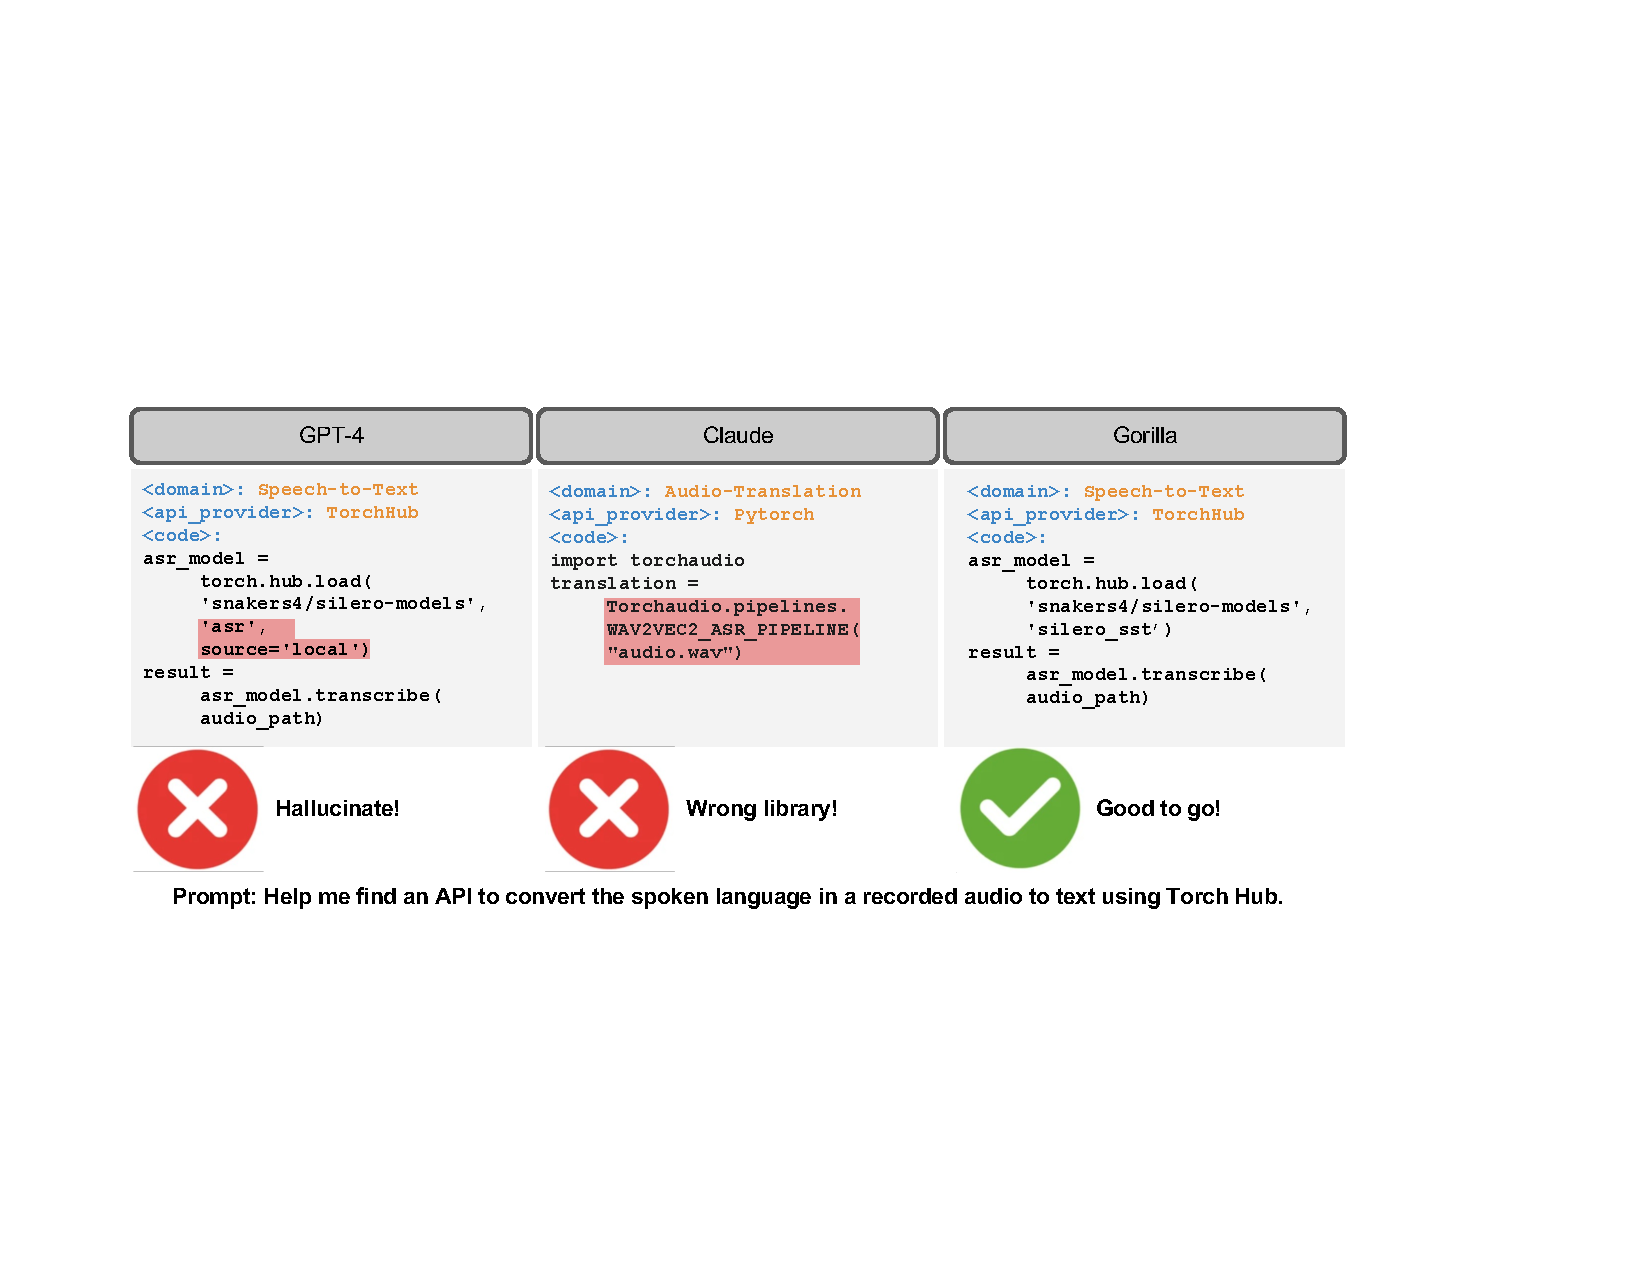
\includegraphics[width=\linewidth]{figures/code-examples.pdf}
\caption{\footnotesize \textbf{Examples of API calls}. Example API calls generated by GPT-4~\cite{openai2023gpt4}, Claude~\cite{Claude}, and \oursmethod{} for the given prompt. In this example, GPT-4 presents a model that doesn't exist, and Claude picks an incorrect library. In contrast, our \oursmethod{} model can identify the task correctly and suggest a fully-qualified API call.}
\label{fig:examplecode}
\end{figure}


In this paper, we explore the use of self-instruct fine-tuning and retrieval to enable LLMs to accurately select from a large, overlapping, and changing set tools expressed using their APIs and API documentation.
We construct, \oursdataset{}, a large corpus of APIs with complex and often overlapping functionality by scraping ML APIs (models) from public model hubs.  
We choose three major model hubs for dataset construction: TorchHub, TensorHub and HuggingFace. We exhaustively include every API call in TorchHub (94 API calls) and TensorHub (696 API calls); For HuggingFace, since the models come in a large number and lots of the models don't have a specification, we choose the most downloaded 20 models per task category (in a total of 925). We also generate 10 synthetic user question prompts per API using Self-Instruct~\cite{wang2022self}. Thus, each entry in the dataset becomes an instruction reference API pair. We adopt a common AST sub-tree matching technique to evaluate the functional correctness of the generated API. We first parse the generated code into an AST tree, then find a sub-tree whose root node is the API call that we care about (e.g., \texttt{torch.hub.load}) and use it to index our dataset. We check the functional correctness and hallucination problem for the LLMs, reporting the corresponding accuracy. 

We then finetune \oursmethod{}, a LLaMA-7B-based model with document retrieval using our dataset. We find that \oursmethod{} significantly outperforms GPT-4 in terms of API functionality accuracy as well as reducing hallucination errors. We show an example output in Fig.~\ref{fig:examplecode}.  Further, our retrieval-aware training of \gorilla{} enables the model to adapt to changes in the API documentation. Finally, we demonstrate Gorilla's ability to understand and reason about constraints.



\begin{figure}[t]
    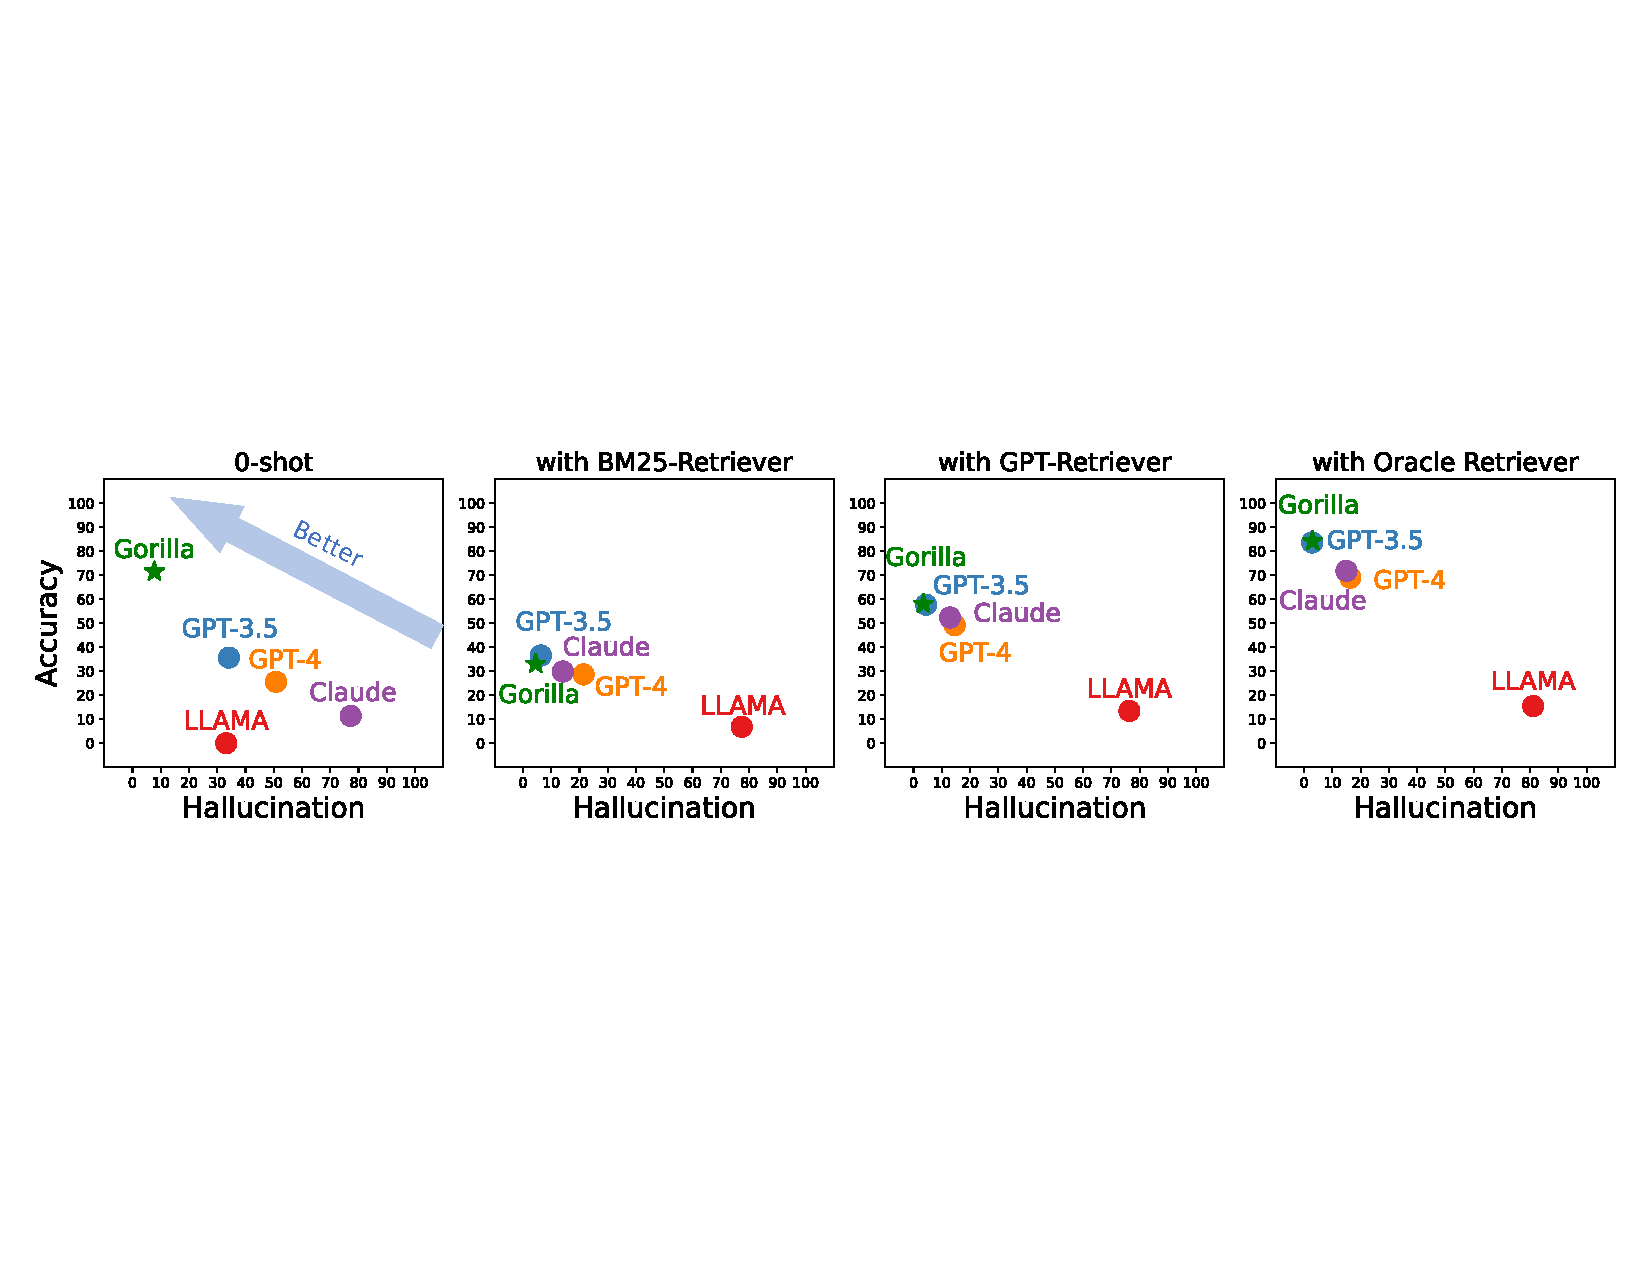
\includegraphics[width=\linewidth]{figures/average_grid.pdf}
\caption{\footnotesize \textbf{Accuracy (vs) hallucination} in four settings, that is,  \emph{zero-shot} (i.e., without any retriever), and \emph{with retrievers}. \texttt{BM25} and \texttt{GPT} are commonly used retrievers and the \texttt{oracle} retriever returns relevant documents at 100\%, indicating an upper bound. Higher in the graph (higher accuracy) and to the left is better (lower hallucination). Across the entire dataset, our model, \oursmethod{}, improves accuracy while reducing hallucination.}
\label{fig:acc-hallu}
\end{figure}



%auto-ignore

\section{Related Work}
There is a long history of pre-training general language representations, and we briefly review the most widely-used approaches in this section.


\subsection{Unsupervised Feature-based Approaches}
Learning widely applicable representations of words has been an active area of research for decades, including non-neural~\cite{brown-etal:1992:_class, ando-zhang:2005, blitzer-mcdonald-pereira:2006:_domain} and neural~\cite{mikolov-etal:2013, pennington-socher-manning:2014:_glove} methods. Pre-trained word embeddings are an integral part of modern NLP systems, offering significant improvements over embeddings learned from scratch~\cite{turian-ratinov-bengio:2010:_word_repres}. To pre-train word embedding vectors, left-to-right language modeling objectives have been used~\cite{minh09}, as well as objectives to  discriminate correct from incorrect words in left and right context~\cite{mikolov-etal:2013}.

These approaches have been generalized to coarser granularities, such as sentence embeddings~\cite{kiros-etal:2015:_skip, logeswaran2018an} or paragraph embeddings~\cite{le-mikolov:2014:_distr}. To train sentence representations, prior work has used objectives to rank candidate next sentences  \cite{DBLP:journals/corr/JerniteBS17, logeswaran2018an},  left-to-right generation of next sentence words given a representation of the previous sentence~\cite{kiros-etal:2015:_skip}, or denoising auto-encoder derived objectives~\cite{hill16}.

%
\begin{figure*}[t!]
%\small
\begin{center}
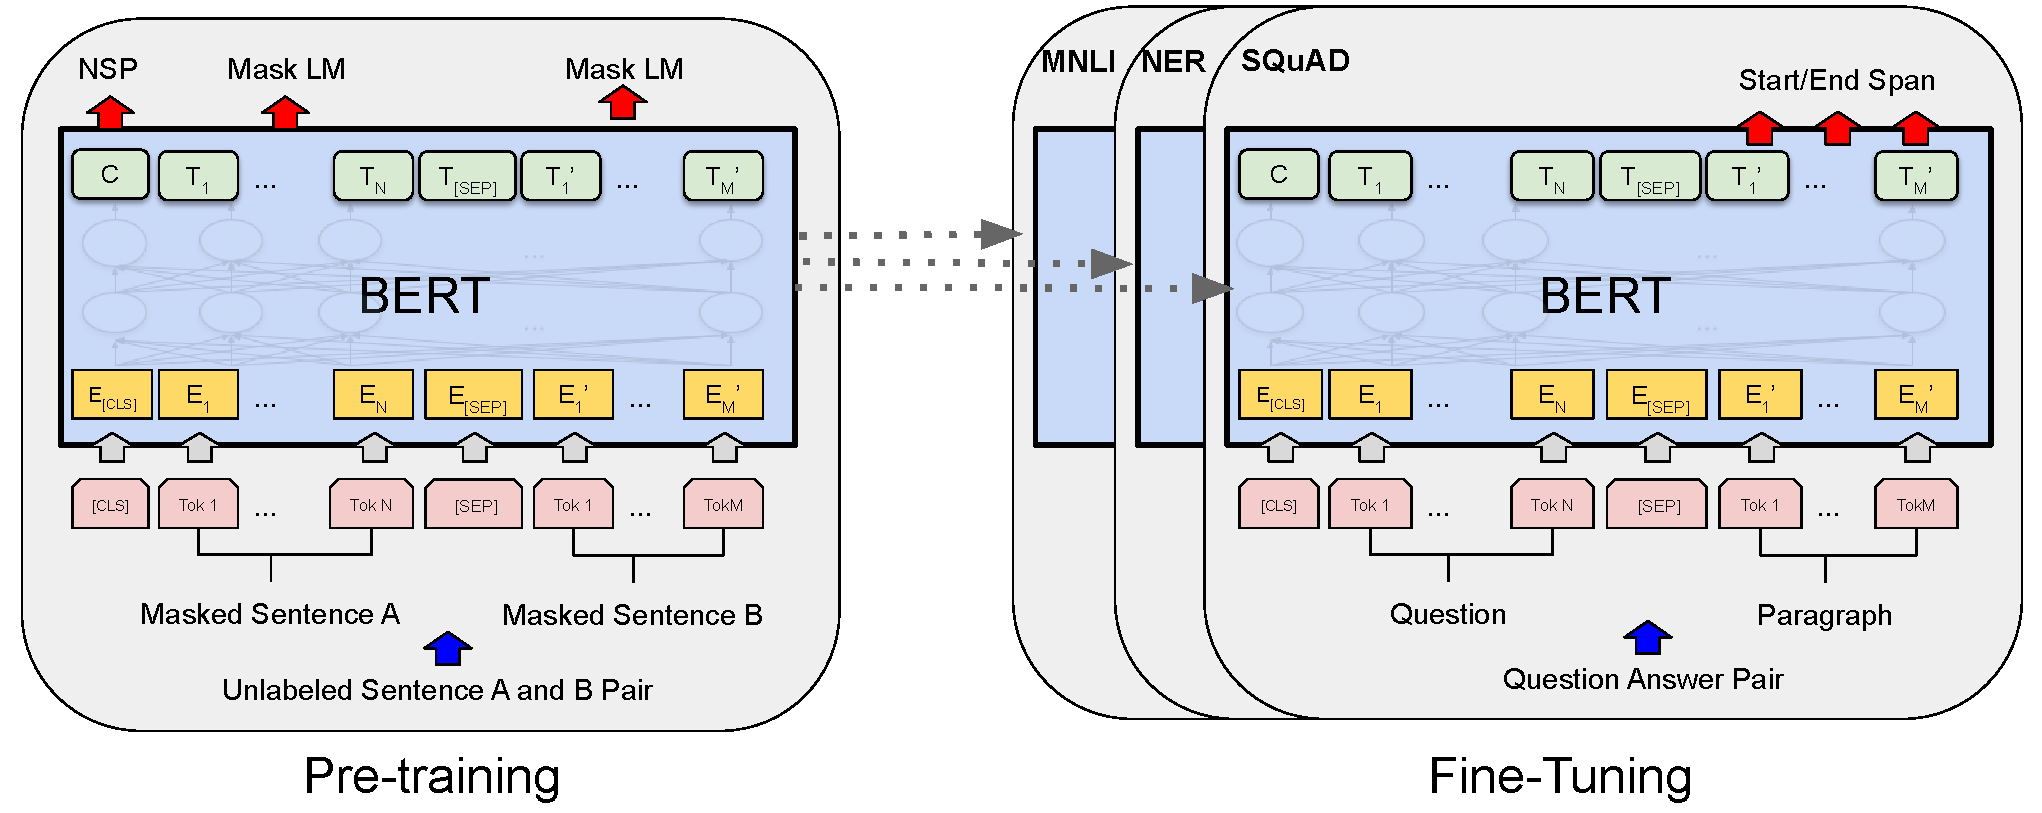
\includegraphics[width=1\textwidth]{BERT_Overall.pdf}
\end{center}
\caption{Overall pre-training and fine-tuning procedures for BERT. Apart from output layers, the same architectures are used in both pre-training and fine-tuning. The same pre-trained model parameters are used to initialize models for different down-stream tasks.  During fine-tuning, all parameters are fine-tuned. {\tt [CLS]} is a special symbol added
in front of every input example, and {\tt [SEP]} is a special separator token (e.g. separating  questions/answers).}
\label{fig:bert_overall}
\end{figure*}
%



ELMo and its predecessor~\cite{peters-etal:2017:_semi, peters-etal:2018:_deep} generalize traditional word embedding research along a different dimension. They extract \emph{context-sensitive} features from a left-to-right and a right-to-left language model. The contextual representation of each token is the concatenation of the left-to-right and right-to-left representations. When integrating contextual word embeddings with existing task-specific architectures, ELMo advances the state of the art for several major NLP benchmarks~\cite{peters-etal:2018:_deep} including question answering~\cite{rajpurkar-etal:2016:_squad}, sentiment analysis~\cite{socher-etal:2013:_recur}, and named entity recognition~\cite{tjong-de:2003}.
\citet{melamud2016context2vec} proposed learning contextual representations through a task to predict a single word from both left and right context
using LSTMs. Similar to ELMo, their model is feature-based and not deeply bidirectional. 
\citet{fedus2018maskgan} shows that the cloze task can be used to improve the robustness of text generation models. 




\subsection{Unsupervised Fine-tuning Approaches}

As with the feature-based approaches, the first works in this direction only pre-trained word embedding parameters from unlabeled text ~\cite{collobert-weston:2008}.  

More recently, sentence or document encoders which produce contextual token representations have been pre-trained from unlabeled text and fine-tuned for a supervised downstream task~\cite{dai-le:2015:_semi, howard-ruder:2018, radford-etal:2018}.  The advantage of these approaches is that few parameters need to be learned from scratch. At least partly due to this advantage, OpenAI GPT~\cite{radford-etal:2018} achieved previously state-of-the-art results on many sentence-level tasks from the GLUE benchmark~\cite{wang-etal:2018:_glue}.  Left-to-right language modeling and auto-encoder objectives have been used for pre-training such models~\cite{howard-ruder:2018, radford-etal:2018,dai-le:2015:_semi}.





\subsection{Transfer Learning from Supervised Data}

There has also been work showing effective transfer from supervised tasks with large datasets, such as natural language inference~\cite{conneau-EtAl:2017:EMNLP2017} and machine translation~\cite{mccann-etal:2017:_learn_trans}. 
Computer vision research has also demonstrated the importance of transfer learning from large pre-trained models, where an effective recipe is to fine-tune models pre-trained with ImageNet~\cite{imagenet_cvpr09, yosinski2014transferable}. 




\section{\model{}: Synergizing \texttt{Re}asoning + \texttt{Act}ing}
\label{sec:react}








Consider a general setup of an agent interacting with an environment for task solving. At time step $t$, an agent receives an observation $o_t \in \mathcal{O}$ from the environment and takes an action $a_t \in \mathcal{A}$ following some policy $\pi(a_t | c_t)$, where $c_t = (o_1, a_1, \cdots, o_{t-1}, a_{t-1}, o_t)$ is the \textit{context} to the agent. Learning a policy is challenging when the mapping $c_t \mapsto a_t$ is highly implicit and requires extensive computation. 
For example, the agent shown in Figure~\ref{fig:teaser}(1c) is unable to generate the correct final action (Act 4) to finish the QA task as it requires complex reasoning over the trajectory context (Question, Act 1-3, Obs 1-3).
Similarly, the agent shown in Figure~\ref{fig:teaser}(2a) fails to comprehend from the context that sinkbasin 1 does not contain peppershaker 1, thus keep producing hallucinating actions.


The idea of \model{} is simple: we augment the agent's action space to $\mathcal{\hat{A}} = \mathcal{A} \cup \mathcal{L}$, where $\mathcal{L}$ is the space of language. An action $\hat{a}_t \in \mathcal{L}$ in the language space, which we will refer to as a \textit{thought} or a \textit{reasoning trace}, does not affect the external environment, thus leading to no observation feedback. Instead, a thought $\hat{a}_t$ aims to compose useful information by reasoning over the current context $c_t$, and update the context $c_{t+1} = (c_t, \hat{a}_t)$ to support future reasoning or acting. 
As shown in Figure~\ref{fig:teaser}, there could be various types of useful thoughts, e.g.\,decomposing task goals and create action plans (2b, Act 1; 1d, Thought 1), injecting commonsense knowledge relevant to task solving (2b, Act 1), extracting important parts from observations (1d, Thought2, 4), track progress and transit action plans (2b, Act 8), handle exceptions and adjust action plans (1d, Thought 3), and so on. 


However, as the language space $\mathcal{L}$ is unlimited, learning in this augmented action space is difficult and requires strong language priors. In this paper, we mainly focus on 
the setup where a frozen large language model, PaLM-540B~\citep{chowdhery2022palm}\footnote{We show some GPT-3~\citep{brown2020language} results in Appendix~\ref{sec:gpt3}, which outperforms PaLM-540B. }, is prompted with few-shot in-context examples to generate both domain-specific actions and free-form language thoughts for task solving (Figure~\ref{fig:teaser} (1d), (2b)). Each in-context example is a human trajectory of actions, thoughts, and environment observations to solve a task instance (see Appendix~\ref{sec:prompts}). 
For the tasks where reasoning is of primary importance (Figure~\ref{fig:teaser}(1)), we alternate the generation of thoughts and actions so that the task-solving trajectory consists of multiple thought-action-observation steps.
In contrast, for  decision making tasks that potentially involve a large number of actions (Figure~\ref{fig:teaser}(2)), thoughts only need to appear sparsely in the most relevant positions of a trajectory, so we let the language model decide the asynchronous occurrence of thoughts and actions for itself.

Since decision making and reasoning capabilities are integrated into a large language model, \model{} enjoys several unique features:
    \textbf{A) Intuitive and easy to design}: Designing \model{} prompts is straightforward as human annotators just type down their thoughts in language on top of their actions taken. No ad-hoc format choice, thought design, or example selection is used in this paper. We detail prompt design for each task in Sections~\ref{sec:knowledge} and \ref{decision_making_tasks}.
    \textbf{B) General and flexible}: Due to the flexible thought space and thought-action occurrence format, \model{} works for diverse tasks with distinct action spaces and reasoning needs, including but not limited to QA, fact verification, text game, and web navigation.
    \textbf{C) Performant and robust}: \model{} shows strong generalization to new task instances while learning solely from one to six in-context examples, consistently outperforming baselines with only reasoning or acting across different domains. We also show in Section~\ref{sec:knowledge} additional benefits when finetuning is enabled, and in Section~\ref{decision_making_tasks} how \model{} performance is robust to prompt selections.
    \textbf{D) Human aligned and controllable}: \model{} promises an interpretable sequential decision making and reasoning process where humans can easily inspect reasoning and factual correctness. Moreover, humans can also control or correct the agent behavior on the go by thought editing, as shown in Figure~\ref{fig:edit} in Section~\ref{decision_making_tasks}.
































\section{Evaluation}
\label{sec:eval}
We carried out an array of experiments on our collected dataset, benchmarking our model \gorilla{} with other models, and exploring how different retrieval methods may impact the performance of the model in making API calls. We then demonstrate that \gorilla{} can easily adapt to test-time changes in API documentation. In addition, we assess Gorilla's ability to reason about API calls under constraints. Lastly, we examined how integrating different retrieval methods during training influences the model's final performance.

\paragraph{Baselines} Primarily, we compare \oursmethod{} with state-of-the-art language models in a zero-shot setting. The models under consideration include: GPT-4 by OpenAI, we use the \texttt{gpt-4-0314} checkpoint; GPT-3.5-turbo with the \texttt{gpt-3.5-turbo-0301} checkpoint, both of which are RLHF-tuned model specifically designed for conversation; Claude with \texttt{claude-v1} checkpoint, a language model by Anthropic, renowned for its lengthy context capabilities; LLaMA-7B, a large language model by Meta and the finest open-source model to date.

\paragraph{Retrievers} The term \emph{Zero-shot} (abbreviated as 0-shot in tables) refers to scenarios where no retriever is used. The sole input to the model is the user's natural language prompt. For \texttt{BM25}, we consider each API as a separate document. During retrieval, we use the user's query to search the index and fetch the most relevant (top-1) API. 
This API is concatenated with the user's prompt to query the LLMs. Similarly, GPT-Index refers to the retrieval model \texttt{text-davinci-003} from OpenAI. Like BM25, each API call is indexed as an individual document, and the most relevant document, given a user query, is retrieved and appended to the user prompt. Lastly, we include an Oracle retriever, which serves two purposes: first, to identify the potential for performance improvement through more efficient retrievers, and second, to assist users who know which API to use but may need to help invoking it. 
In all cases, when a retriever is used, it is appended to the user's prompt as follows: \texttt{<user\_prompt>} \texttt{Use this API documentation for reference:} \texttt{<retrieved\_API\_doc\_JSON>}. 
The dataset for these evaluations is detailed in Sec~\ref{sec:method}. We emphasize that we have maintained a holdout test set on which we report our findings. The holdout test set was created by dividing the self-instruct dataset's {instruction, API} pairs into training and testing sets.


\subsection{AST Accuracy on API call}

\begin{figure}[t]
    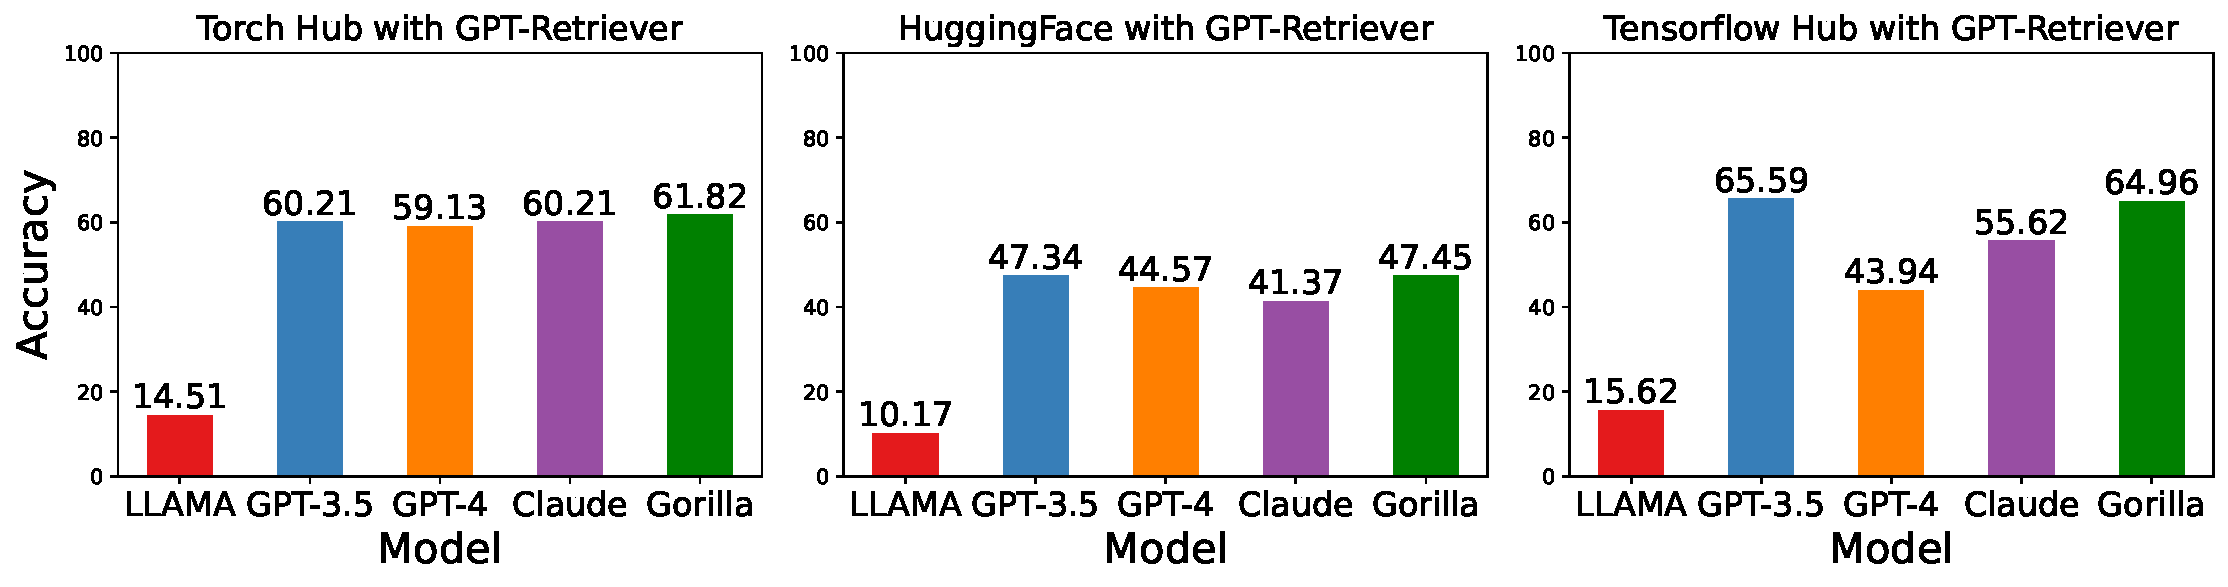
\includegraphics[width=\linewidth]{figures/grid_bars_GPT_Retrieval.pdf}
\caption{\footnotesize \textbf{Accuracy with GPT-retriever.} 
\oursmethod{} outperforms on Torch Hub and Hugging-Face while matching performance on Tensorflow Hub for all existing SoTA LLMs - closed source, and open source. }
\label{fig:images}
\end{figure}
We first demonstrate the results for the AST accuracy for different models. We present the results in Tab.~\ref{tab:llm_eval}. We test each model for different retriever settings defined above. We report the overall accuracy, the error by hallucination and the error by selecting wrong API call. Note that for TorchHub and TensorHub, we evaluate all the models using AST tree accuracy score. However, for HuggingFace, since the dataset is not exhaustive, for all the models except \oursmethod{}, we only check if they can provide the correct domain names. So this problem reduces to picking one of the multiple choices. 


\paragraph{Finetuning without Retrieval} In Tab.~\ref{tab:llm_eval} we show that lightly fine-tuned \oursmethod{} gets the state-of-the-art performance zero-shot over all the models, 20.43\% better than GPT-4 and 10.75\% better than ChatGPT. When compared to other open-source models LLAMA, the improvement is as big as 83\%. his suggests quantitatively, that finetuning is better than retrieval, at-least in our scope. 

In addition, we found that finetuning without retriever and putting ground truth retriever in evaluation time rarely helps the performance: 0.88\% worse in TensorHub and 0.97\% better in HuggingFace. If we put BM25 or GPT-Index as retriever, results will be significantly dropped: 21.50\% in Torch Hub and 47.57\% in HuggingFace. The result illustrates that adding a non-optimal retriever at test time will sometime misguide the model and result in more errors. We will discuss an interesting ablation on how finetuning with the retriever will help the performance in the next paragraph. 





\begin{table*}[h]
    \caption{\small \textbf{Evaluating LLMs on Torch Hub, HuggingFace, and Tensorflow Hub APIs}}
    \label{tab:llm_eval}
     \setlength{\tabcolsep}{10pt} % Default value: 6pt
    \begin{adjustbox}{width=\textwidth}
    \begin{tabular}{l c c c | c c c | c c c}
    \toprule
    
    LLM (retriever) & \multicolumn{3}{c}{TorchHub} & \multicolumn{3}{c}{HuggingFace} & \multicolumn{3}{c}{TensorFlow Hub} \\
    & overall $\uparrow$ & hallu $\downarrow$ & err $\downarrow$ & overall $\uparrow$ & hallu $\downarrow$ & err $\downarrow$ & overall $\uparrow$ & hallu $\downarrow$ & err $\downarrow$ \\
    \midrule
    LLAMA (0-shot) & 0 & 100 & 0 & 0.00 & 97.57 & 2.43 & 0 & 100 & 0 \\
    GPT-3.5 (0-shot) & 48.38 & 18.81 & 32.79 & 16.81 & 35.73 & 47.46 & 41.75 & 47.88 & 10.36 \\
    GPT-4 (0-shot) & 38.70 & 36.55 & 24.7 & 19.80 & 37.16 & 43.03 & 18.20 & 78.65 & 3.13 \\
    Claude (0-shot) & 18.81 & 65.59 & 15.59 & 6.19 & 77.65 & 16.15 & 9.19 & 88.46 & 2.33 \\
    \gorilla{} (0-shot) & \textbf{59.13} & \textbf{6.98} & 33.87 & \textbf{71.68} & \textbf{10.95} & 17.36 & \textbf{83.79} & \textbf{5.40} & 10.80 \\
    \midrule
    LLAMA (BM-25) & 8.60 & 76.88 & 14.51 & 3.00 & 77.99 & 19.02 & 8.90 & 77.37 & 13.72 \\
    GPT-3.5 (BM-25) & 38.17 & 6.98 & 54.83 & \textbf{17.26} & 8.30 & 74.44 & \textbf{54.16} & 3.64 & 42.18 \\
    GPT-4 (BM-25) & 35.48 & 11.29 & 53.22 & 16.48 & 15.93 & 67.59 & 34.01 & 37.08 & 28.90 \\
    Claude (BM-25) & 39.78 & 5.37 & 54.83 & 14.60 & 15.82 & 69.58 & 35.18 & 21.16 & 43.64 \\
    \gorilla{} (BM-25) & \textbf{40.32} & \textbf{4.30} & 55.37 & 17.03 & \textbf{6.42} & 76.55 & 41.89 & \textbf{2.77} & 55.32 \\
    \midrule
    LLAMA (GPT-Index) & 14.51 & 75.8 & 9.67 & 10.18 & 75.66 & 14.20 & 15.62 & 77.66 & 6.71 \\
    GPT-3.5 (GPT-Index) & 60.21 & 1.61 & 38.17 & 29.08 & 7.85 & 44.80 & \textbf{65.59} & 3.79 & 30.50 \\
    GPT-4 (GPT-Index) & 59.13 & 1.07 & 39.78 & 44.58 & 11.18 & 44.25 & 43.94 & 31.53 & 24.52 \\
    Claude (GPT-Index) & 60.21 & 3.76 & 36.02 & 41.37 & 18.81 & 39.82 & 55.62 & 16.20 & 28.17 \\
    \gorilla{} (GPT-Index) & \textbf{61.82} & \textbf{0} & 38.17 & \textbf{47.46} & \textbf{8.19} & 44.36 & 64.96 & \textbf{2.33} & 32.70 \\
    \midrule
    LLAMA (Oracle) & 16.12 & 79.03 & 4.83 & 17.70 & 77.10 & 5.20 & 12.55 & 87.00 & 0.43 \\
    GPT-3.5 (Oracle) & 66.31 & 1.60 & 32.08 & 89.71 & 6.64 & 3.65 & \textbf{95.03} & \textbf{0.29} & 4.67 \\
    GPT-4 (Oracle) & 66.12 & 0.53 & 33.33 & 85.07 & 10.62 & 4.31 & 55.91 & 37.95 & 6.13 \\
    Claude (Oracle) & 63.44 & 3.76 & 32.79 & 77.21 & 19.58 & 3.21 & 74.74 & 21.60 & 3.64 \\
    \gorilla{} (Oracle) & \textbf{67.20} & \textbf{0} & 32.79 & \textbf{91.26} & \textbf{7.08} & 1.66 & 94.16 & 1.89 & 3.94 \\
    \bottomrule
    \end{tabular}
    \end{adjustbox}
\end{table*}



\paragraph{Finetuning with Retrieval} We now discuss an interesting experiment on how finetuning language with retriever incorporated is helping the performance. The settings for this experiment are finetuning the base LLAMA with the prompt (instruction generated), reference API document (from golden-truth oracle), and the example output generated by GPT-4. In Tab.~\ref{tab:retrieve}, we can see that incorporating ground truth retriever in the finetuning pipeline achieves significantly better results 12.37\% better than training without retriever in Torch Hub and 23.46\% better in HuggingFace. However, we found that at evaluation time, current retrievers still have a big gap between the ground truth retriever: using GPT-Index at evaluation results in 29.20\% accuracy degradation, and using BM25 results in a 52.27\% accuracy degradation. Nevertheless, we can still conclude that with a better retriever, finetuning with retriever is still a better method to adopt while in another scenario, when a good retriever is not available, zero-shot finetuning might be the preferred choice.

\begin{table*}[h]
    \caption{\small \textbf{Comparison of retrieval techniques}
    }
    \label{tab:retrieve}
     \setlength{\tabcolsep}{10pt} % Default value: 6pt
    \begin{adjustbox}{width=\textwidth}
    \begin{tabular}{l cccc | cccc}
    \toprule
    & \multicolumn{4}{c}{\gorilla{} without Retriever} & \multicolumn{4}{c}{\oursmethod{} with Oracle retriever} \\ 
     % \cmidrule(lr){4-23}
     \midrule
    & zero-shot & BM25 & GPT-Index & Oracle & zero-shot & BM25 & GPT-Index & Oracle  \\
    \midrule
    Torch Hub (overall) $\uparrow$ & 59.13 & 37.63 & 60.21 & 54.83 & 0 & 40.32 & 61.82 & 67.20  \\
    HuggingFace (overall) $\uparrow$ & 71.68 & 11.28 & 28.10 & 45.58 & 0 & 17.04 & 47.46 & 91.26  \\
    TensorHub (overall)  $\uparrow$ & 83.79 & 34.30 & 52.40 & 82.91 & 0 & 41.89 & 64.96 & 94.16 \\
    \midrule
    Torch Hub (Hallu) $\downarrow$ & 6.98 & 11.29 & 4.30 & 15.59 & 100 & 4.30 & 0 & 0  \\
    HuggingFace (Hallu) $\downarrow$ & 10.95 & 46.46 & 41.48 & 52.77 & 99.67 & 6.42 & 8.19 & 7.08  \\
    TensorHub (Hallu) $\downarrow$ & 5.40 & 20.43 & 19.70 & 13.28 & 100 & 2.77 & 2.33 & 1.89\\
    \bottomrule
    \end{tabular}
    \end{adjustbox}
\end{table*}

\paragraph{Hallucination with LLM} One phenomenon we observe is that zero-shot prompting with LLMs (GPT-4/GPT-3.5) to call APIs results in dire hallucination errors. These errors, while diverse, commonly manifest in erroneous behavior such as the model invoking the "AutoModel.from\_pretrained(dir\_name)" command with arbitrary GitHub repository names. Surprisingly, we also found that in TorchHub, HuggingFace and TensorFlow Hub, GPT-3.5 has less hallucination errors than GPT-4. This finding is also consistent for the settings when various retrieving methods are provided: 0-shot, BM25, GPT-Index and the oracle. This might suggest that RLHF plays a central role in turning the model to be truthful. Additional examples and discussion are in Appendix.

\subsection{Test-Time Documentation Change}

\begin{figure}[t]
    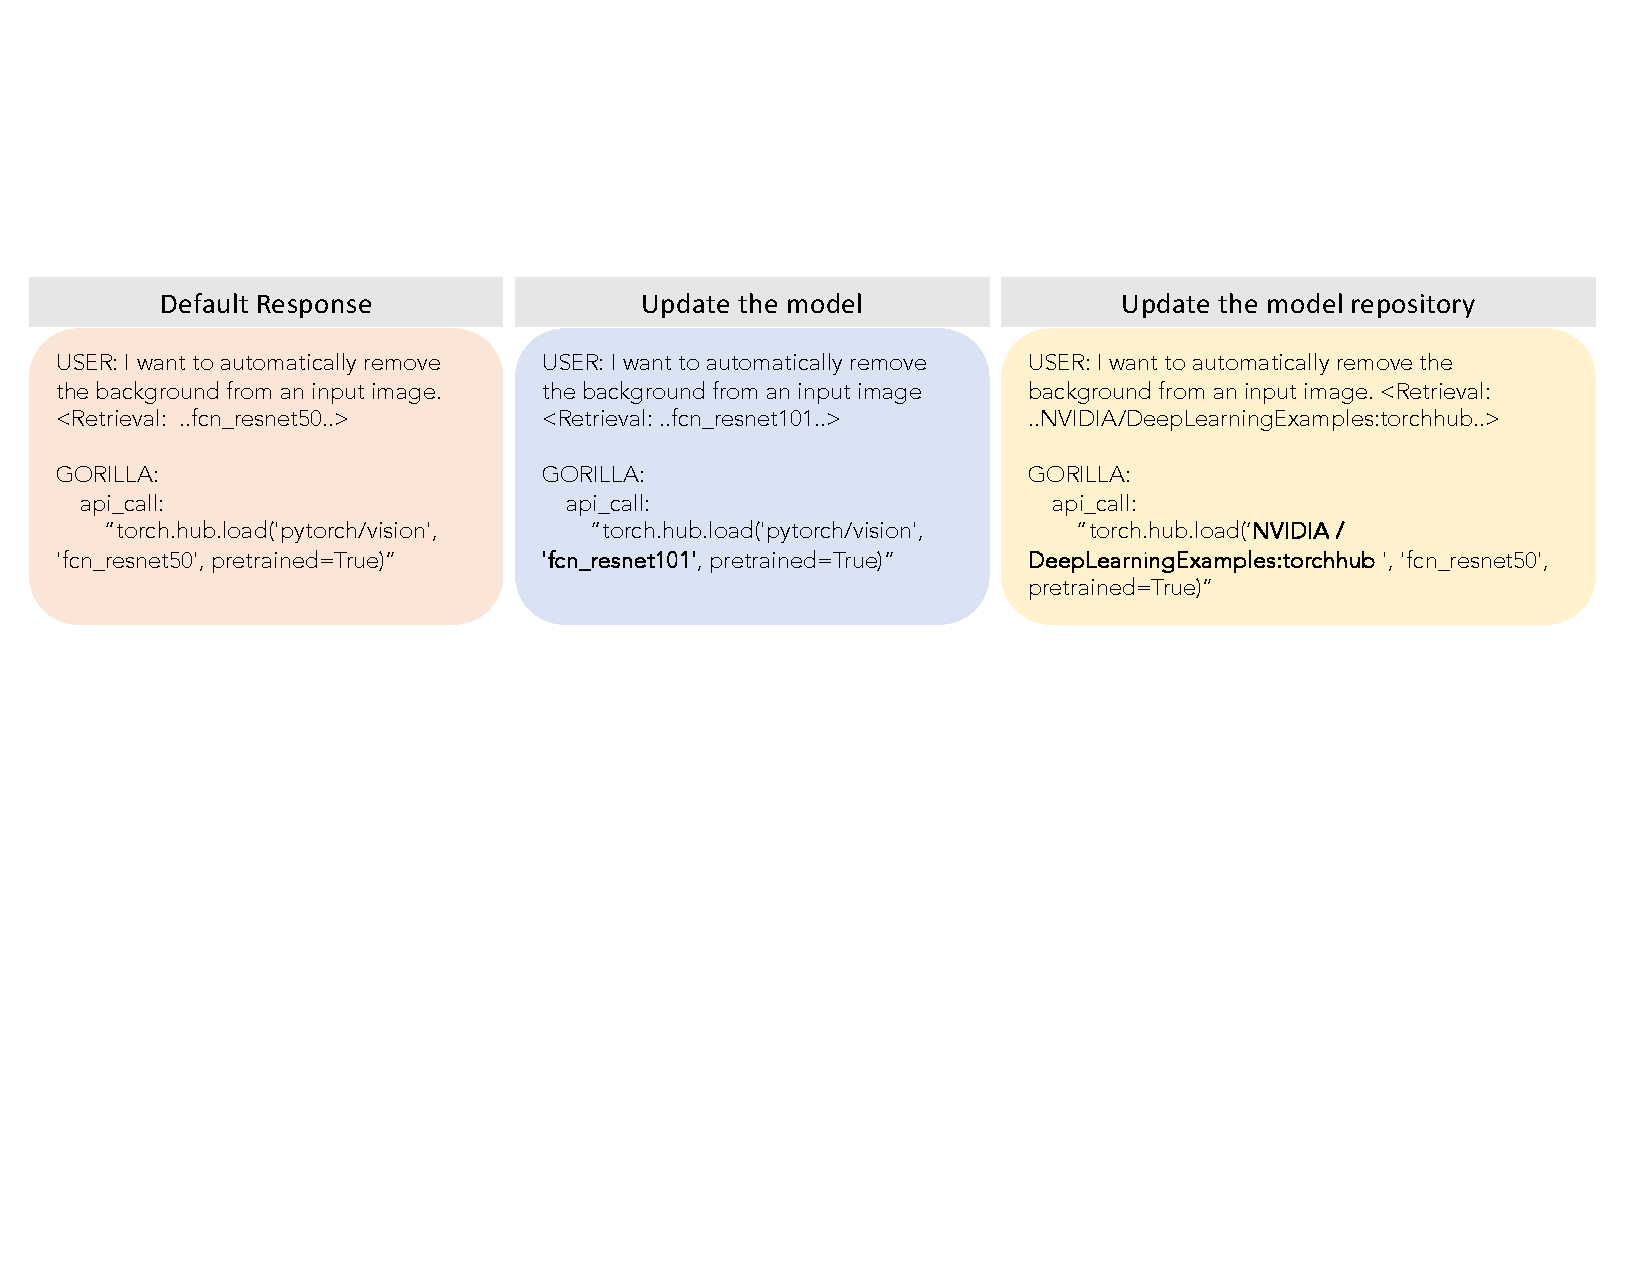
\includegraphics[width=\linewidth]{figures/docu.pdf}
\caption{\footnotesize \textbf{Gorilla's retriever\---aware training enables it to react to changes in the APIs.} The second column demonstrates changes in model \- upgrading FCN's ResNet\---50 backbone to ResNet\---101. The third column demonstrate changes in model registry from \texttt{pytorch/vision} to \texttt{NVIDIA/DeepLearningExamples:torchhub} }
\label{fig:docu}
\end{figure}


The rapidly evolving nature of API documentation presents a significant challenge for the application of LLMs in this field. These documents are often updated at a frequency that outpaces the re-training or fine-tuning schedule of LLMs, making these models particularly brittle to changes in the information they are designed to process. This mismatch in update frequency can lead to a decline in the utility and reliability of LLMs over time.

However, with the introduction of Gorilla's retriever-aware training, we can readily adapt to changes in API documentation. This novel approach allows the model to remain updated and relevant, even as the API documentation it relies on undergoes modifications. This is a pivotal advancement in the field, as it ensures that the LLM maintains its efficacy and accuracy over time, providing reliable outputs irrespective of changes in the underlying documentation.

For instance, consider the scenario illustrated in Figure 6, where the training of Gorilla has allowed it to react effectively to changes in APIs. This includes alterations such as upgrading the FCN's ResNet-50 backbone to ResNet-101, as demonstrated in the second column of the figure. This capability ensures that the LLM remains relevant and accurate even as the underlying models and systems undergo upgrades and improvements.
Furthermore, the third column in Figure 6 shows how Gorilla adapts to changes in the model registry from \texttt{pytorch/vision} to \texttt{NVIDIA/DeepLearningExamples:torchhub}. This reflects the model's ability to adjust to shifts in API sources, which is vital as organizations may change their preferred model registries over time.

In summary, Gorilla's ability to adapt to test-time changes in API documentation offers numerous benefits. It maintains its accuracy and relevance over time, adapts to the rapid pace of updates in API documentation, and adjusts to modifications in underlying models and systems. This makes it a robust and reliable tool for API calls, significantly enhancing its practical utility.



\subsection{API Call with Constraints}
We now focus on the language model's capability of understanding constraints. For any given task, which API call to invoke is typically a tradeoff between a multitude of factors. In the case of RESTFul APIs, it could be the cost of each invocation (\$), and the latency of response (ms), among others. Similarly, within the scope of ML APIs, it is desirable for \gorilla{} to respect constraints such as accuracy, number of learnable parameters in the model, the size on disk, peak memory consumption, FLOPS, etc. We present the underlying ablation study evaluating the ability of different models in zero-shot and with retrievers settings to respect a given accuracy constraint. This setting is best understood with an example. If the user were to ask for an Image classification model that achieves at least 80\% top-1 accuracy on the Imagenet dataset, then while both are classification models hosted by Torch Hub,    \texttt{ResNeXt-101 32x16d} with a top-1 accuracy of 84.2\% would be the right model whose API to call and not, say, \texttt{MobileNetV2} which has a top-1 accuracy of 71.88\%. 

\begin{table*}[h]
    \caption{\small \textbf{Evaluating LLMs on constraint-aware API invocations}
    }
    \label{tab:const}
    \begin{adjustbox}{max width=\textwidth}
    \begin{tabular}{l cccc|cccc|cccccc}
    \toprule
    & \multicolumn{4}{c}{GPT-3.5} & \multicolumn{4}{c}{GPT-4} & \multicolumn{4}{c}{\oursmethod{}}\\ 
     % \cmidrule(lr){4-23}
     \midrule
    & 0-shot & BM25 & GPT-Index & Oracle & 0-shot & BM25 & GPT-Index & Oracle & 0-shot & BM25 & GPT-Index & Oracle \\
    \midrule
    Torch Hub (overall) &  \textbf{73.94} & 62.67 & 81.69 & 80.98 & 62.67 & 56.33 & 71.11 & 69.01  & 71.83 & 57.04 & 71.83 & 78.16 \\
    Torch Hub (Hallu) &  19.01 & 30.98 & 14.78 & 14.08 & \textbf{15.49} & 27.46 & \textbf{14.08} & \textbf{9.15} & 19.71 & 39.43 & 26.05 & 16.90 \\
    Torch Hub (err) &  7.04 & 6.33 & 3.52 & 4.92 & 21.83 & 16.19 & 14.78 & 21.83 & 8.45 & 3.52 & 2.11 & 4.92 \\
    \midrule
    Accuracy const & 43.66 & \textbf{33.80} & \textbf{33.09} & 69.01 & 43.66 & 29.57 & 29.57 & 59.15 & \textbf{47.88} & 30.28 & 26.76 & 67.60\\
    \midrule
    & \multicolumn{4}{c}{LLAMA} & \multicolumn{4}{c}{Claude}\\ 
     % \cmidrule(lr){4-23}
     \midrule
      % \cmidrule{1-9}
    & 0-shot & BM25 & GPT-Index & Oracle & 0-shot & BM25 & GPT-Index & Oracle  \\
    % \midrule
    \cmidrule{1-9}
    Torch Hub (overall) &  0 & 8.45 & 11.97 & 19.71 & 29.92 & \textbf{81.69} & \textbf{82.39} & \textbf{81.69}\\
    Torch Hub (Hallu) &   100 & 91.54 & 88.02 & 78.87 & 67.25 & \textbf{16.19} & 15.49 & 13.38\\
    Torch Hub (err) &  0 & 0 & 0 & 1.4  & 2.81 & 2.11 & 2.11 & 4.92\\
    % \midrule
     \cmidrule{1-9}
    Accuracy const & 0 & 6.33 & 3.52 & 17.60 & 17.25 & 29.57 & 31.69 & \textbf{69.71}\\
    \bottomrule
    \end{tabular}
    \end{adjustbox}
\end{table*}

For Table~\ref{tab:const}, we filtered a subset of the Torch Hub dataset that had accuracy defined for at least one-dataset in its model card (65.26\% of TorchHub dataset in Table~\ref{tab:llm_eval}). We notice that with constraints, understandably, the accuracy drops across all models, with and without a retriever. \gorilla{} is able to match performance with the best-performing model GPT-3.5 when using retrievals (BM25, GPT-Index) and has the highest accuracy in the Zero-shot case. This highlights Gorilla's ability to navigate APIs while considering the trade-offs between different constraints. 



% Describe limitations and any potential negative societal impacts


In this paper, we answer the question \emph{can we enhance open-source LLMs to compete with leading closed LLM APIs in tool manipulation, with practical amount of human supervision}. 
Drawing from our observations of the common tool manipulation failures and insights from the literature on conventional NLP tasks with LLM, we propose to instantiate model alignment with programmatical data generation, system prompts, and in-context demonstration retrievers to improve the tool manipulation capability of open-source models.
To comprehensively evaluate the impact of these techniques, we create the \textit{\snact}, a benchmark consisting of diverse software tools for real-world tasks. 
Our results demonstrate that these techniques can make the leading open-source LLMs competitive with the OpenAI GPT-4 in $4$ out of $8$ \snact\  tasks, all achieved with a practical amount of human labeling effort.


\section{Limitations \& Social Impacts}
\label{sec:limitation}

With the goal of wanting to have a challenging dataset, we chose ML APIs, given their functional similarity. The potential downside to APIs that focus on the ML domain, is their propensity to produce biased predictions if trained on skewed data, potentially disadvantaging certain sub-groups. To counter this concern and foster a deeper understanding of these APIs, we are releasing our extensive dataset, consisting of over 11,000 instruction-API pairs. This resource will serve the wider community as a valuable tool for studying and benchmarking existing APIs, contributing to a more fair and optimized usage of machine learning.
\section{Acknowledgement}
\label{sec:ack}
This research is supported in part by gifts to UC Berkley Sky Computing Lab from Astronomer, Google, IBM, Intel, Lacework, Microsoft, Nexla, Samsung SDS, Uber, and VMware.


\bibliographystyle{apalike}
\bibliography{references}

\newpage
\section{Additional Results}
\subsection{GPT-3 Experiments} 
\label{sec:gpt3}
\begin{table}[ht]
    \centering
\begin{tabular}{c | cc}
\toprule
 & PaLM-540B & GPT-3 \\ \midrule
HotpotQA (exact match) & 29.4 & \textbf{30.8} \\
ALFWorld (success rate \%) & 70.9 & \textbf{78.4} \\ 
\bottomrule
\end{tabular}%
    \caption{\model{} prompting results using PaLM-540B vs.\,GPT-3 (text-davinci-002, greedy decoding). On HotpotQA, we randomly sample a subset of 500 validation questions. On ALFWorld, we use all 134 unseen validation task instances, and use the best prompt set according to PaLM-540B.}
    \label{tab:gpt3}
\end{table}
We run additional GPT-3~\citep{brown2020language} experiments to confirm \model{} prompting performance is general across different large language models. As shown in Table~\ref{tab:gpt3}, GPT-3 (text-davinci-002, greedy decoding) consistently outperforms PaLM-540B on HotpotQA and ALFWorld, possibly because it is finetuned with human instruction following. This indicates ReAct prompting is effective across different large language models on different tasks.
The code for these experiments are at \url{https://react-lm.github.io/}.
\subsection{\model{} obtains up-to-date knowledge on HotpotQA}
\begin{figure}[ht]
    \centering
    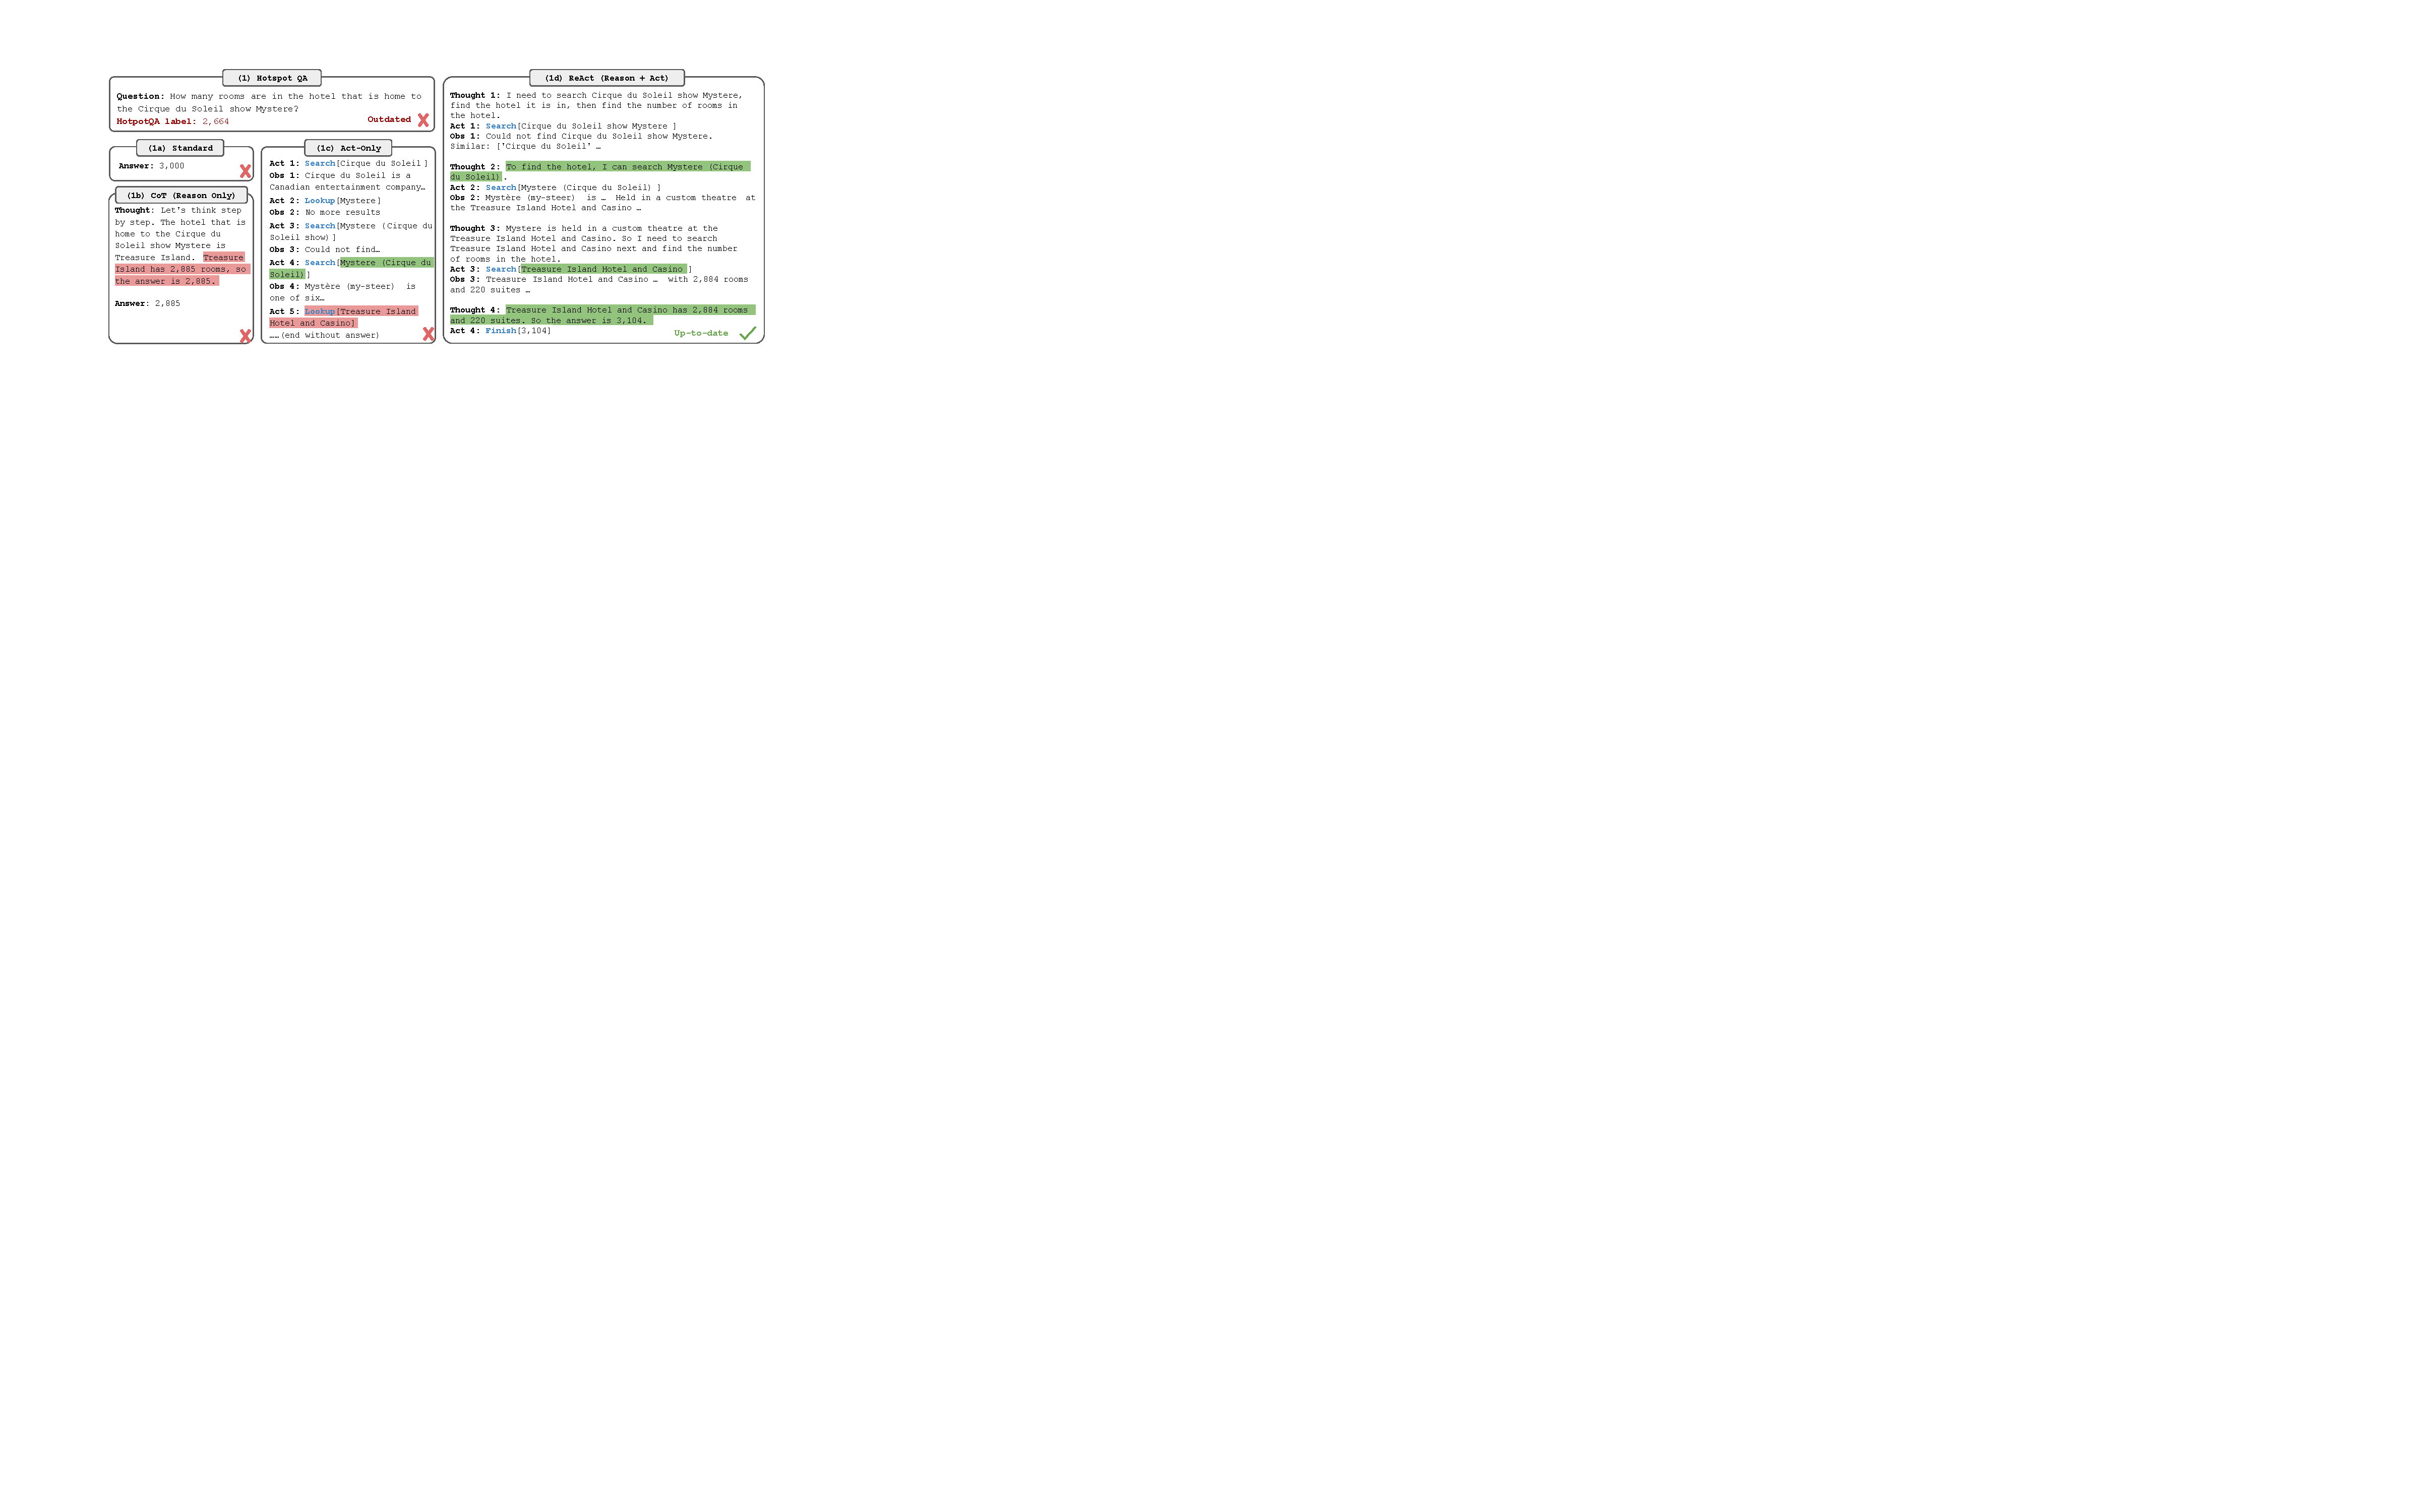
\includegraphics[width=\textwidth]{iclr2023/figure/date.pdf}
    \caption{
    {
    Another example HotpotQA question, where the original label is outdated. Only \model{} is able to obtain the up-to-date answer thanks to real-world web interaction plus reasoning.}
    }
    \label{fig:date}
    \vspace{-10pt}
\end{figure}

During trajectory inspection, we also find that sometimes \model{} does not agree with dataset labels as the labels themselves could be outdated. For example, as shown in Figure~\ref{fig:date}, the question asks about the size of a hotel, which increased from the HotpotQA construction time. While \palm{} and \reason{} give wrong answers due to hallucination, \act{} fails despite the access of real-world web interaction, due to a lack of reasoning to guide how to interact with the Internet for QA. Only \model{} is able to retrieve up-to-date information from the Internet and provide a reasonable answer. Therefore, better incorporation of reasoning abilities might benefit recent Internet-augmented language models~\citep{nakano2021webgpt,lazaridou2022internet,shuster2022language} for up-to-date task solving. 
\subsection{Human-in-the-loop behavior correction on AlfWorld} 
\begin{figure}[ht]
    \centering
    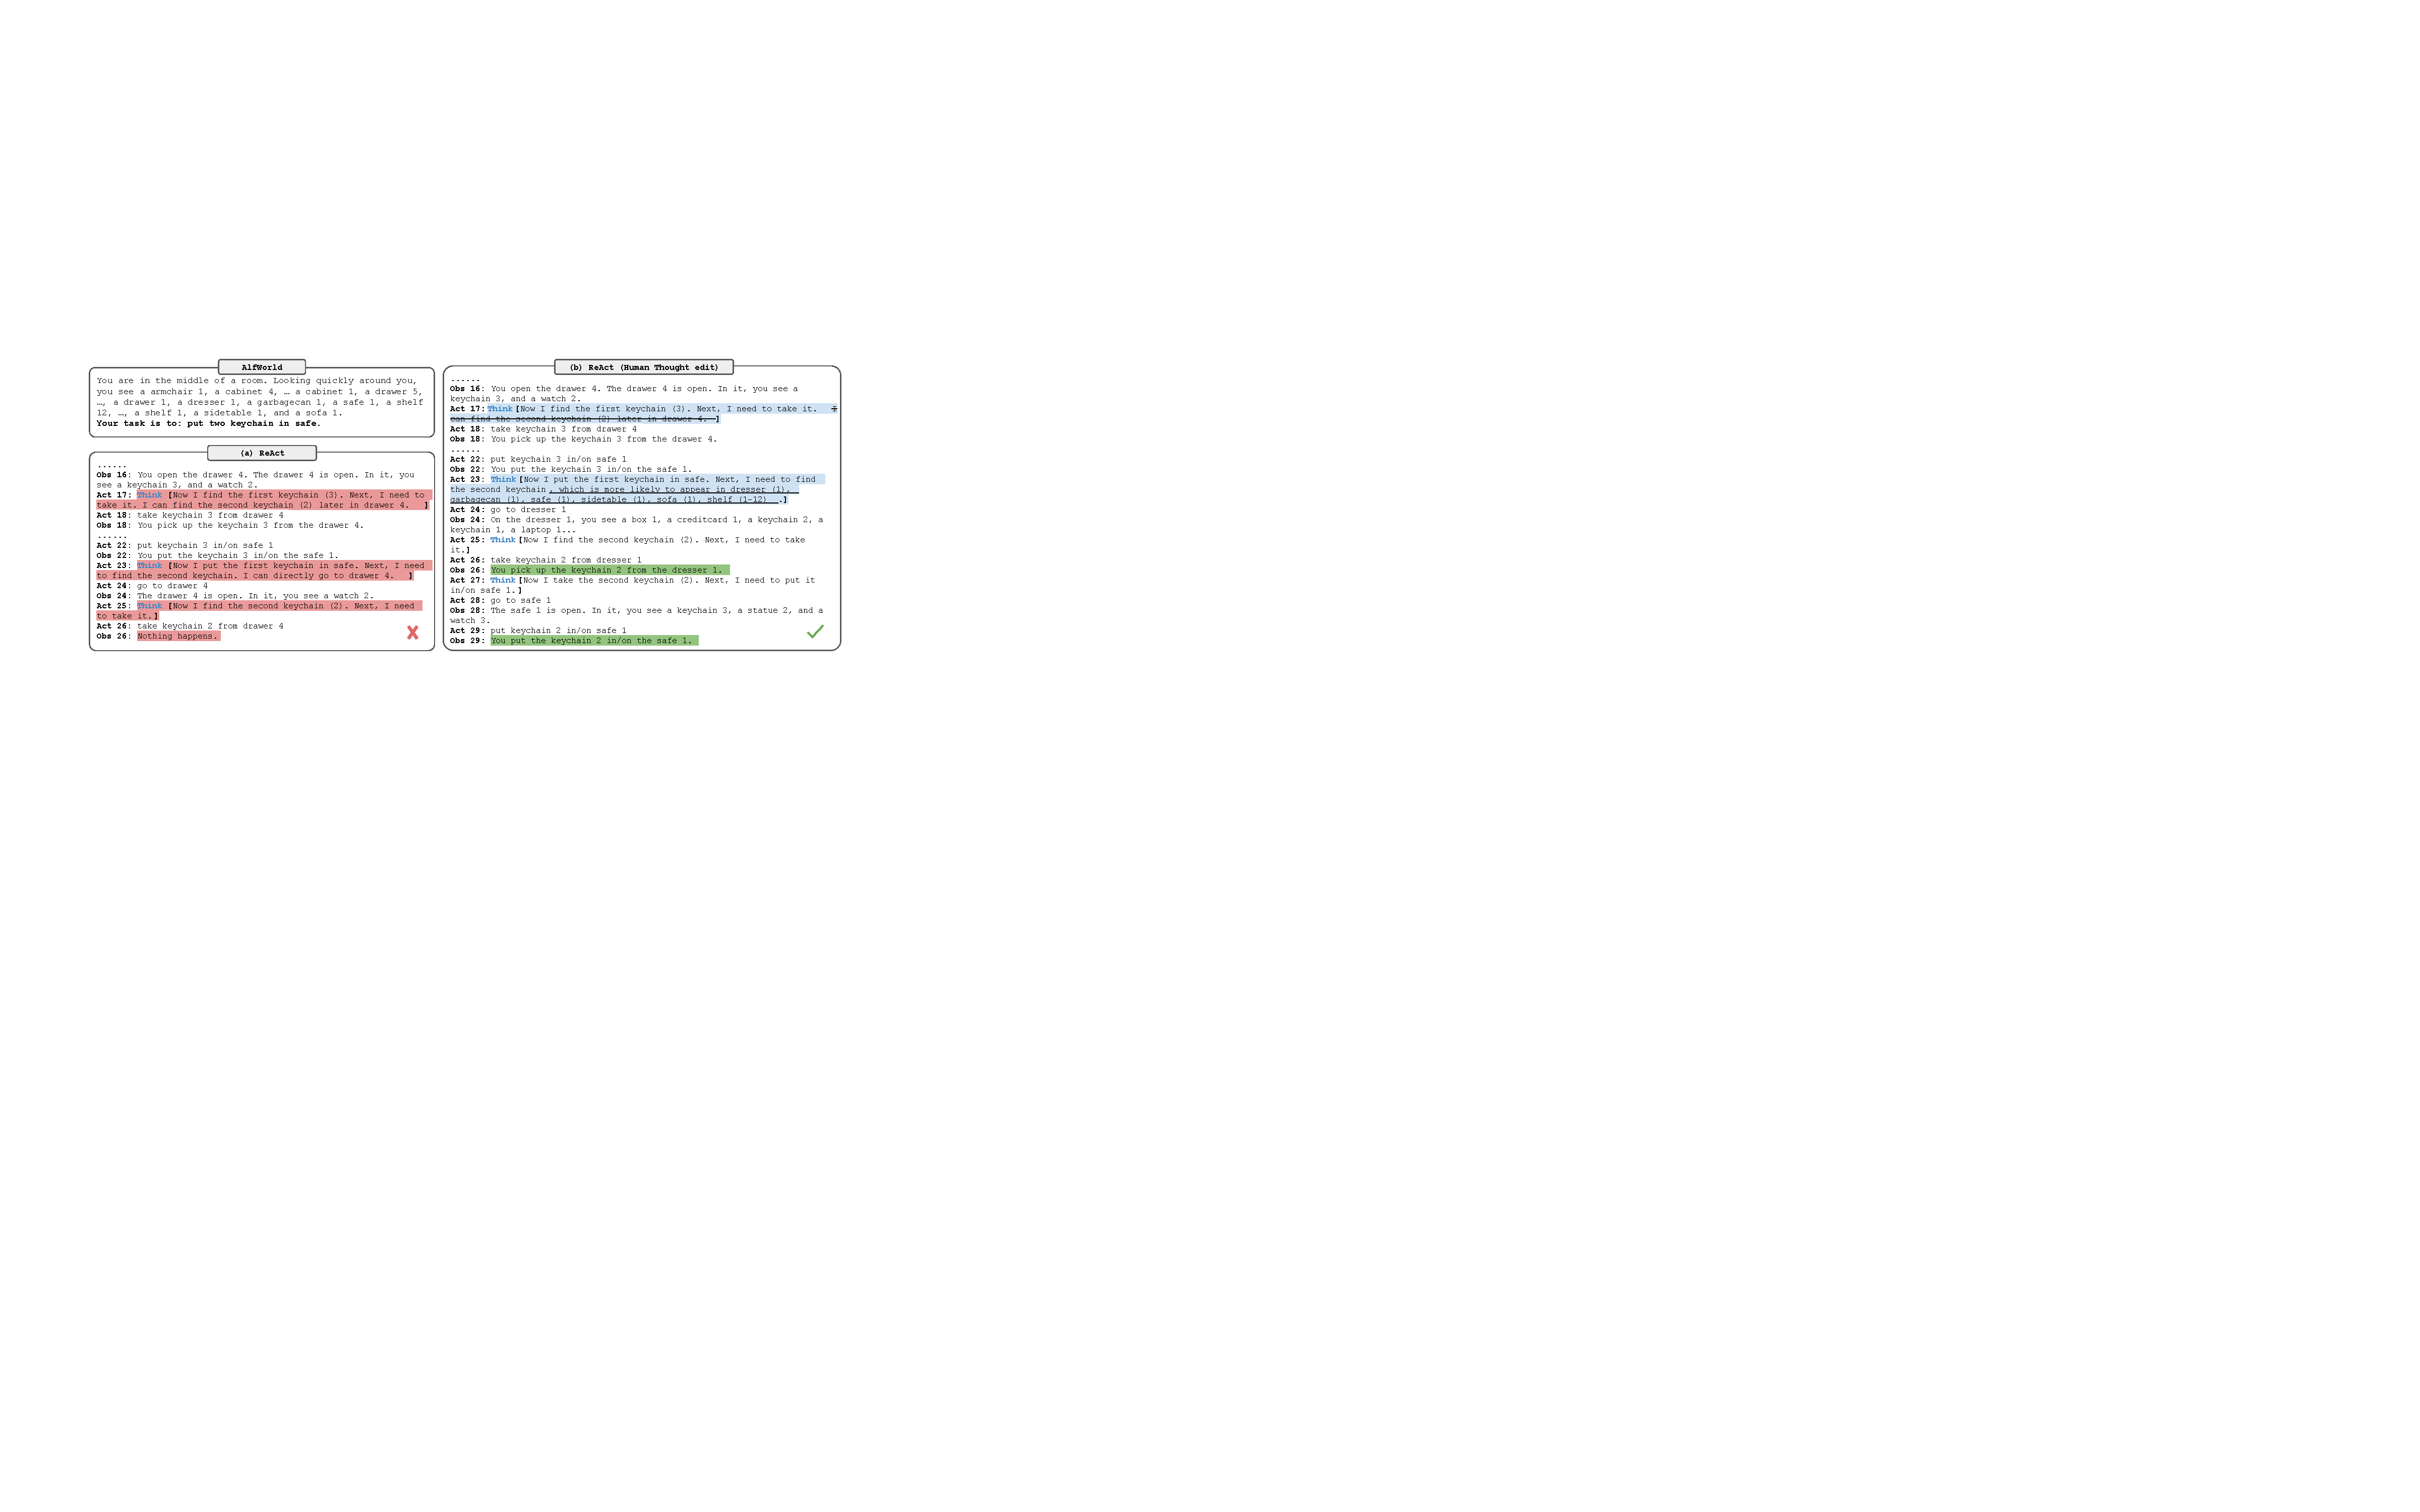
\includegraphics[width=\textwidth]{iclr2023/figure/human_edit.pdf}
    \caption{
    A human-in-the-loop behavior correction example with \model{} in AlfWorld. 
    (a) \model{} trajectory fails due to a hallucinating thought (Act 17).
    (b) By a human simply editing two thoughts (Act 17, 23), the \model{} trajectory produces desirable reasoning traces and actions and succeeds.
    }
    \label{fig:edit}
    \vspace{-10pt}
\end{figure}

We also explore human-in-the-loop interaction with \model{}, to allow a human to inspect and edit \model's reasoning traces. Figure~\ref{fig:edit} shows that
by simply removing a hallucinating sentence in Act 17 and adding some hints in Act 23, \model{} can be made to change its behavior drastically to align with these human thought edits and succeed in the task. 
From a human perspective, solving such a task becomes significantly easier, from typing tens of actions to only editing a couple of thoughts, which enables new forms of human-machine collaboration.
We note that such a policy edit on-the-go is difficult for \act{} and previous RL methods, as a human cannot change the model parameters, and changing a few actions might not edit the rest of the model behavior. 
This paradigm is also more than human dialogue to update the goal or subgoal as in \citet{huang2022inner} --- while editing \model{} thoughts can do these, it can also modify the model's internal belief, reasoning styles, or anything the flexible thought space supports, for better task solving. 
We believe this is an exciting direction for human alignment and leave more systematic study as future work.

\section{Experiment Details}
\subsection{HotpotQA Finetuning Details}
\label{sec:hotpot_finetune}
For all finetuning we use a batch size of 64.
On PaLM-8B, we finetune \model{} and \act{} methods for $4,000$ steps and \palm{} and \reason{} methods for $2,000$ steps. 
On PaLM-62B, we finetune \model{} and \act{} methods for $4,000$ steps and \palm{} and \reason{} methods for $1,000$ steps. 
We find \model{} and \act{} methods generally benefit from more training steps (and more training data), while  \palm{} and \reason{} methods degrade soon after finetuning.

\subsection{AlfWorld IM-Style Details}
\label{sec:alfworld_im}
For the IM-style ablation, the same expert trajectories used in \model{} are reannotated with dense external feedback thoughts within these trajectories, that limit \modelim{} to only think about (1) decomposing the current goal and (2) the current subgoal that needs to be completed. In particular, \modelim{} lacks thoughts that (1) determine when a subgoal is completed (2) determine what the next subgoal should be (3) inducing the LLM to refer to its internal pretraining knowledge to identify where items can be within the environment. 


\section{Prompts}
\label{sec:prompts}
\subsection{HotpotQA}
\begin{table}[H]
\scriptsize
\begin{minipage}{0.9\linewidth}
Hotpot QA Prompts
\centering
\ttfamily
\begin{tabular}{l p{0.9\linewidth}}
\midrule
\sethlcolor{cyan}\hl{Original} & \\
Question &  What is the elevation range for the area that the eastern sector of the Colorado orogeny extends into? \\
Answer &  1,800 to 7,000 ft\\
\\
Question &  Musician and satirist Allie Goertz wrote a song about the "The Simpsons" character Milhouse, who Matt Groening named after who?\\
Answer &  Richard Nixon\\
\\
Question &  Which documentary is about Finnish rock groups, Adam Clayton Powell or The Saimaa Gesture?\\
Answer &  The Saimaa Gesture\\
\\
Question &  What profession does Nicholas Ray and Elia Kazan have in common?\\
Answer &  director, screenwriter, actor\\
\\
Question &  Which magazine was started first Arthur's Magazine or First for Women?\\
Answer &  Arthur's Magazine\\
\\
Question &  Were Pavel Urysohn and Leonid Levin known for the same type of work?\\
Answer &  Yes\\


\midrule
\sethlcolor{red}\hl{\act} & \\
Question &  What is the elevation range for the area that the eastern sector of the Colorado orogeny extends into?\\
Action 1 &  Search[Colorado orogeny]\\
Observation 1 &  The Colorado orogeny was an episode of mountain building (an orogeny) in Colorado and surrounding areas.\\
Action 2 &  Lookup[eastern sector]\\
Observation 2 &  (Result 1 / 1) The eastern sector extends into the High Plains and is called the Central Plains orogeny.\\
Action 3 &  Search[High Plains]\\
Observation 3 &  High Plains refers to one of two distinct land regions: \\
Action 4 &  Search[High Plains (United States)]\\
Observation 4 &  The High Plains are a subregion of the Great Plains. From east to west, the High Plains rise in elevation from around 1,800 to 7,000 ft (550 to 2,130 m).[3]\\
Action 5 &  Finish[1,800 to 7,000 ft]\\
\\
Question &  Musician and satirist Allie Goertz wrote a song about the "The Simpsons" character Milhouse, who Matt Groening named after who?\\
Action 1 &  Search[Milhouse]\\
Observation 1 &  Milhouse Mussolini Van Houten is a recurring character in the Fox animated television series The Simpsons voiced by Pamela Hayden and created by Matt Groening.\\
Action 2 &  Lookup[named after]\\
Observation 2 &  (Result 1 / 1) Milhouse was named after U.S. president Richard Nixon, whose middle name was Milhous. \\
Action 3 &  Finish[Richard Nixon]\\
\\
Question &  Which documentary is about Finnish rock groups, Adam Clayton Powell or The Saimaa Gesture?\\
Action 1 &  Search[Adam Clayton Powell]\\
Observation 1 &  Could not find [Adam Clayton Powell]. Similar:  ['Adam Clayton Powell III', 'Seventh Avenue (Manhattan)', 'Adam Clayton Powell Jr. State Office Building', 'Isabel Washington Powell', 'Adam Powell', 'Adam Clayton Powell (film)', 'Giancarlo Esposito'].\\
Action 2 &  Search[Adam Clayton Powell (film)]\\
Observation 2 &  Adam Clayton Powell is a 1989 American documentary film directed by Richard Kilberg. The film is about the rise and fall of influential African-American politician Adam Clayton Powell Jr.[3][4] It was later aired as part of the PBS series The American Experience.\\
Action 3 &  Finish[The Saimaa Gesture]\\
\\
Question &  What profession does Nicholas Ray and Elia Kazan have in common?\\
Action 1 &  Search[Nicholas Ray]\\
Observation 1 &  Nicholas Ray (born Raymond Nicholas Kienzle Jr., August 7, 1911 – June 16, 1979) was an American film director, screenwriter, and actor best known for the 1955 film Rebel Without a Cause.\\
Action 2 &  Search[Elia Kazan]\\
Observation 2 &  Elia Kazan was an American film and theatre director, producer, screenwriter and actor.\\


\midrule \multicolumn{2}{r}{\textit{Continued on next page}} \\
\end{tabular}
\end{minipage}%
\end{table}


\begin{table}[H]
\scriptsize
\begin{minipage}{0.9\linewidth}
Hotpot QA Prompts -- Continued from previous page
\centering
\ttfamily
\begin{tabular}{l p{0.9\linewidth}}
\midrule
\\
Action 3 &  Finish[director, screenwriter, actor]\\
Question &  Which magazine was started first Arthur's Magazine or First for Women?\\
Action 1 &  Search[Arthur's Magazine]\\
Observation 1 &  Arthur's Magazine (1844--1846) was an American literary periodical published in Philadelphia in the 19th century. \\
Action 2 &  Search[First for Women]\\
Observation 2 &  First for Women is a woman's magazine published by Bauer Media Group in the USA.[1] The magazine was started in 1989. \\
Action 3 &  Finish[Arthur's Magazine]\\
\\
Question &  Were Pavel Urysohn and Leonid Levin known for the same type of work?\\
Action 1 &  Search[Pavel Urysohn]\\
Observation 1 &  Pavel Samuilovich Urysohn (February 3, 1898 - August 17, 1924) was a Soviet mathematician who is best known for his contributions in dimension theory.\\
Action 2 &  Search[Leonid Levin]\\
Observation 2 &  Leonid Anatolievich Levin is a Soviet-American mathematician and computer scientist. \\
Action 3 &  Finish[yes]\\
\midrule
\sethlcolor{green}\hl{\reason} & \\
Question &  What is the elevation range for the area that the eastern sector of the Colorado orogeny extends into?\\
Thought &  Let's think step by step. The eastern sector of Colorado orogeny extends into the High Plains. High Plains rise in elevation from around 1,800 to 7,000 ft, so the answer is 1,800 to 7,000 ft.\\
Answer &  1,800 to 7,000 ft\\
\\
Question &  Musician and satirist Allie Goertz wrote a song about the "The Simpsons" character Milhouse, who Matt Groening named after who?\\
Thought &  Let's think step by step. Milhouse was named after U.S. president Richard Nixon, so the answer is Richard Nixon.\\
Answer &  Richard Nixon\\
\\
Question &  Which documentary is about Finnish rock groups, Adam Clayton Powell or The Saimaa Gesture?\\
Thought &  Let's think step by step. Adam Clayton Powell (film) is a documentary about an African-American politician, not Finnish rock groups. So the documentary about Finnish rock groups must instead be The Saimaa Gesture.\\
Answer &  The Saimaa Gesture\\
\\
Question &  What profession does Nicholas Ray and Elia Kazan have in common?\\
Thought &  Let's think step by step. Professions of Nicholas Ray are director, screenwriter, and actor. Professions of Elia Kazan are director, producer, screenwriter, and actor. So profession Nicholas Ray and Elia Kazan have in common is director, screenwriter, and actor.\\
Answer &  director, screenwriter, actor\\
\\
Question &  Which magazine was started first Arthur's Magazine or First for Women?\\
Thought &  Let's think step by step. Arthur's Magazine was started in 1844. First for Women was started in 1989. 1844 (Arthur's Magazine) < 1989 (First for Women), so Arthur's Magazine was started first.\\
Answer &  Arthur's Magazine\\
\\
Question &  Were Pavel Urysohn and Leonid Levin known for the same type of work?\\
Thought &  Let's think step by step. Pavel Urysohn is a mathematician. Leonid Levin is a mathematician and computer scientist. So Pavel Urysohn and Leonid Levin have the same type of work.\\
Answer &  Yes\\


\midrule
\sethlcolor{yellow}\hl{\model} & \\
Question &  What is the elevation range for the area that the eastern sector of the Colorado orogeny extends into?\\
Thought 1 &  I need to search Colorado orogeny, find the area that the eastern sector of the Colorado orogeny extends into, then find the elevation range of the area.\\
Action 1 &  Search[Colorado orogeny]\\
Observation 1 &  The Colorado orogeny was an episode of mountain building (an orogeny) in Colorado and surrounding areas.\\
Thought 2 &  It does not mention the eastern sector. So I need to look up eastern sector.\\
Action 2 &  Lookup[eastern sector]\\
Observation 2 &  (Result 1 / 1) The eastern sector extends into the High Plains and is called the Central Plains orogeny.\\
Thought 3 &  The eastern sector of Colorado orogeny extends into the High Plains. So I need to search High Plains and find its elevation range.\\
Action 3 &  Search[High Plains]\\
Observation 3 &  High Plains refers to one of two distinct land regions  \\
Thought 4 &  I need to instead search High Plains (United States).\\
Action 4 &  Search[High Plains (United States)]\\

\midrule \multicolumn{2}{r}{\textit{Continued on next page}} \\

\end{tabular}
\end{minipage}%
\end{table}


\begin{table}[H]
\scriptsize
\begin{minipage}{0.9\linewidth}
Hotpot QA Prompts -- Continued from previous page
\centering
\ttfamily
\begin{tabular}{l p{0.9\linewidth}}
\midrule
\\
Observation 4 &  The High Plains are a subregion of the Great Plains. From east to west, the High Plains rise in elevation from around 1,800 to 7,000 ft (550 to 2,130 m).[3]\\
Thought 5 &  High Plains rise in elevation from around 1,800 to 7,000 ft, so the answer is 1,800 to 7,000 ft.\\
Action 5 &  Finish[1,800 to 7,000 ft]\\
\\
Question &  Musician and satirist Allie Goertz wrote a song about the "The Simpsons" character Milhouse, who Matt Groening named after who?\\
Thought 1 &  The question simplifies to "The Simpsons" character Milhouse is named after who. I only need to search Milhouse and find who it is named after.\\
Action 1 &  Search[Milhouse]\\
Observation 1 &  Milhouse Mussolini Van Houten is a recurring character in the Fox animated television series The Simpsons voiced by Pamela Hayden and created by Matt Groening.\\
Thought 2 &  The paragraph does not tell who Milhouse is named after, maybe I can look up "named after".\\
Action 2 &  Lookup[named after]\\
Observation 2 &  (Result 1 / 1) Milhouse was named after U.S. president Richard Nixon, whose middle name was Milhous. \\
Thought 3 &  Milhouse was named after U.S. president Richard Nixon, so the answer is Richard Nixon.\\
Action 3 &  Finish[Richard Nixon]\\
\\
Question &  Which documentary is about Finnish rock groups, Adam Clayton Powell or The Saimaa Gesture?\\
Thought 1 &  I need to search Adam Clayton Powell and The Saimaa Gesture, and find which documentary is about Finnish rock groups.\\
Action 1 &  Search[Adam Clayton Powell]\\
Observation 1 &  Could not find [Adam Clayton Powell]. Similar:  ['Adam Clayton Powell III', 'Seventh Avenue (Manhattan)', 'Adam Clayton Powell Jr. State Office Building', 'Isabel Washington Powell', 'Adam Powell', 'Adam Clayton Powell (film)', 'Giancarlo Esposito'].\\
Thought 2 &  To find the documentary, I can search Adam Clayton Powell (film).\\
Action 2 &  Search[Adam Clayton Powell (film)]\\
Observation 2 &  Adam Clayton Powell is a 1989 American documentary film directed by Richard Kilberg.
The film is about the rise and fall of influential African-American politician Adam Clayton Powell Jr.[3][4] It was later aired as part of the PBS series The American Experience.\\
Thought 3 &  Adam Clayton Powell (film) is a documentary about an African-American politician, not Finnish rock groups. So the documentary about Finnish rock groups must instead be The Saimaa Gesture.\\
Action 3 &  Finish[The Saimaa Gesture]\\
\\
Question &  What profession does Nicholas Ray and Elia Kazan have in common?\\
Thought 1 &  I need to search Nicholas Ray and Elia Kazan, find their professions, then find the profession they have in common.\\
Action 1 &  Search[Nicholas Ray]\\
Observation 1 &  Nicholas Ray (born Raymond Nicholas Kienzle Jr., August 7, 1911 – June 16, 1979) was an American film director, screenwriter, and actor best known for the 1955 film Rebel Without a Cause.\\
Thought 2 &  Professions of Nicholas Ray are director, screenwriter, and actor. I need to search Elia Kazan next and find his professions.\\
Action 2 &  Search[Elia Kazan]\\
Observation 2 &  Elia Kazan was an American film and theatre director, producer, screenwriter and actor.\\
Thought 3 &  Professions of Elia Kazan are director, producer, screenwriter, and actor. So profession Nicholas Ray and Elia Kazan have in common is director, screenwriter, and actor.\\
Action 3 &  Finish[director, screenwriter, actor]\\
\\
Question &  Which magazine was started first Arthur's Magazine or First for Women?\\
Thought 1 &  I need to search Arthur's Magazine and First for Women, and find which was started first.\\
Action 1 &  Search[Arthur's Magazine]\\
Observation 1 &  Arthur's Magazine (1844-1846) was an American literary periodical published in Philadelphia in the 19th century. \\
Thought 2 &  Arthur's Magazine was started in 1844. I need to search First for Women next.\\
Action 2 &  Search[First for Women]\\
Observation 2 &  First for Women is a woman's magazine published by Bauer Media Group in the USA.[1] The magazine was started in 1989. \\
Thought 3 &  First for Women was started in 1989. 1844 (Arthur's Magazine) < 1989 (First for Women), so Arthur's Magazine was started first.\\
Action 3 &  Finish[Arthur's Magazine]\\
\\
Question &  Were Pavel Urysohn and Leonid Levin known for the same type of work?\\
Thought 1 &  I need to search Pavel Urysohn and Leonid Levin, find their types of work, then find if they are the same.\\
Action 1 &  Search[Pavel Urysohn]\\

\midrule \multicolumn{2}{r}{\textit{Continued on next page}} \\



\end{tabular}
\end{minipage}%
\end{table}


\begin{table}[H]
\scriptsize
\begin{minipage}{0.9\linewidth}
Hotpot QA Prompts -- Continued from previous page
\centering
\ttfamily
\begin{tabular}{l p{0.9\linewidth}}
\midrule
Observation 1 &  Pavel Samuilovich Urysohn (February 3, 1898 - August 17, 1924) was a Soviet mathematician who is best known for his contributions in dimension theory.\\
Thought 2 &  Pavel Urysohn is a mathematician. I need to search Leonid Levin next and find its type of work.\\
Action 2 &  Search[Leonid Levin]\\
Observation 2 &  Leonid Anatolievich Levin is a Soviet-American mathematician and computer scientist. \\
Thought 3 &  Leonid Levin is a mathematician and computer scientist. So Pavel Urysohn and Leonid Levin have the same type of work. \\
Action 3 &  Finish[yes]\\
\bottomrule
\end{tabular}
\end{minipage}%
\end{table}



\subsection{Fever}
\begin{table}[H]
\scriptsize
\begin{minipage}{0.9\linewidth}
FEVER Prompts
\centering
\ttfamily
\begin{tabular}{l p{0.9\linewidth}}
\midrule
\sethlcolor{cyan}\hl{Original} &   Determine if there is Observation that SUPPORTS or REFUTES a Claim, or if there is NOT ENOUGH INFORMATION. \\
\\
\\
Claim & Nikolaj Coster-Waldau worked with the Fox Broadcasting Company.\\
Answer & SUPPORTS\\
\\
\\
Claim & Stranger Things is set in Bloomington, Indiana.\\
Answer & REFUTES\\
\\
\\
Claim & Beautiful reached number two on the Billboard Hot 100 in 2003.\\
Answer & NOT ENOUGH INFO\\


\midrule
\sethlcolor{red}\hl{\act} & Determine if there is Observation that SUPPORTS or REFUTES a Claim, or if there is NOT ENOUGH INFORMATION. \\
\\
\\
Claim & Nikolaj Coster-Waldau worked with the Fox Broadcasting Company.\\
Action2 & Search[Nikolaj Coster-Waldau]\\
Observation 1 & Nikolaj William Coster-Waldau (born 27 July 1970) is a Danish actor and producer. He graduated from the Danish National School of Performing Arts in Copenhagen in 1993,[1] and had his breakthrough role in Denmark with the film Nightwatch (1994). He played Jaime Lannister in the HBO fantasy drama series Game of Thrones, for which he received two Primetime Emmy Award nominations for Outstanding Supporting Actor in a Drama Series.. Coster-Waldau has appeared in numerous films in his native Denmark and Scandinavia, including Headhunters (2011) and A Thousand Times Good Night (2013). In the U.S, his debut film role was in the war film Black Hawk Down (2001), playing Medal of Honor recipient Gary Gordon.[2] He then played a detective in the short-lived Fox television series New Amsterdam (2008), and appeared in the 2009 Fox television film Virtuality, originally intended as a pilot.\\
Action 2 & Finish[SUPPORTS]\\
\\
\\
Claim &  Stranger Things is set in Bloomington, Indiana.\\
Action 1 & Search[Stranger Things]\\
Observation 1 &  Stranger Things is an American science fiction horror drama television series created by the Duffer Brothers. Set in the 1980s, primarily in the fictional town of Hawkins, Indiana, the series centers on a number of mysteries and supernatural events occurring around the town and their impact on an ensemble of child and adult characters. \\
Action 2 & Finish[REFUTES]\\
\\\\
Claim &  Beautiful reached number two on the Billboard Hot 100 in 2003.\\
Action 1 & Search[Beautiful]\\
Observation 1 &  Could not find [Beautiful]. Similar: ['Beautiful', 'Beautiful, Beautiful', 'A Beautiful Mind (film)', 'Beautiful (Christina Aguilera song)', 'Life Is Beautiful'].\\
Action 2 & Search[Beautiful (Christina Aguilera song)\\
Observation 2 &  "Beautiful" is a song recorded by American singer Christina Aguilera for her fourth studio album, Stripped (2002).\\
Action 3 & Lookup[Billboard Hot 100]\\
Observation 3 &  (Result 1 / 3) The song peaked at number two on the Billboard Hot 100 in the United States, where it was certified Gold for 500,000 units shipped.\\
Action 4 & Finish[NOT ENOUGH INFO]\\

\midrule
\sethlcolor{green}\hl{\reason} & Determine if there is Observation that SUPPORTS or REFUTES a Claim, or if there is NOT ENOUGH INFORMATION. \\
\\
\\
Claim &  Nikolaj Coster-Waldau worked with the Fox Broadcasting Company.\\
Thought &  Nikolaj William Coster-Waldau appeared in the 2009 Fox television film Virtuality, so he has worked with the Fox Broadcasting Company.\\
Answer &  SUPPORTS\\
\\
\\
Claim &  Stranger Things is set in Bloomington, Indiana.\\
Thought &  Stranger Things is in the fictional town of Hawkins, Indiana, not in Bloomington, Indiana.\\
Answer & REFUTES\\
\midrule \multicolumn{2}{r}{\textit{Continued on next page}} \\


\end{tabular}
\end{minipage}%
\end{table}





\begin{table}[H]
\scriptsize
\begin{minipage}{0.9\linewidth}
\textit{Fever Prompts -- Continued from previous page}
\centering
\ttfamily
\begin{tabular}{l p{0.9\linewidth}}
\midrule
\\
Claim &  Beautiful reached number two on the Billboard Hot 100 in 2003.\\
Thought &  The song peaked at number two on the Billboard Hot 100 in the United States, but not sure if it was in 2003.\\
Answer &  NOT ENOUGH INFO\\
\midrule
\sethlcolor{yellow}\hl{\model} & Determine if there is Observation that SUPPORTS or REFUTES a Claim, or if there is NOT ENOUGH INFORMATION. \\
\\
\\
Claim &  Nikolaj Coster-Waldau worked with the Fox Broadcasting Company.\\
Thought 1 &  I need to search Nikolaj Coster-Waldau and find if he has worked with the Fox Broadcasting Company. \\
Action 1 &  Search[Nikolaj Coster-Waldau]\\
Observation 1 &  Nikolaj William Coster-Waldau (born 27 July 1970) is a Danish actor and producer. He graduated from the Danish National School of Performing Arts in Copenhagen in 1993,[1] and had his breakthrough role in Denmark with the film Nightwatch (1994). He played Jaime Lannister in the HBO fantasy drama series Game of Thrones, for which he received two Primetime Emmy Award nominations for Outstanding Supporting Actor in a Drama Series.. Coster-Waldau has appeared in numerous films in his native Denmark and Scandinavia, including Headhunters (2011) and A Thousand Times Good Night (2013). In the U.S, his debut film role was in the war film Black Hawk Down (2001), playing Medal of Honor recipient Gary Gordon.[2] He then played a detective in the short-lived Fox television series New Amsterdam (2008), and appeared in the 2009 Fox television film Virtuality, originally intended as a pilot.\\
Thought 2 &  Because he "appeared in the 2009 Fox television film Virtuality", he should have worked with the Fox Broadcasting Company.\\
Action 2 &  Finish[SUPPORTS]\\
\\
\\
Claim &  Stranger Things is set in Bloomington, Indiana.\\
Thought 1 & I should search for Stranger Things, and see if it is set in Bloomington, Indiana.\\
Action 1 & Search[Stranger Things]\\
Observation 1 &  Stranger Things is an American science fiction horror drama television series created by the Duffer Brothers. Set in the 1980s, primarily in the fictional town of Hawkins, Indiana, the series centers on a number of mysteries and supernatural events occurring around the town and their impact on an ensemble of child and adult characters. \\
Thought 2 & The observation says that it is set in a "fictional town of Hawkins, Indiana", so it is not set in Bloomington.\\
Action 2 & Finish[REFUTES]\\
\\
\\
Claim &  Beautiful reached number two on the Billboard Hot 100 in 2003.\\
Thought 1 & I need to search the song Beautiful and find if it reached number two on the Billboard Hot 100 in 2003.\\
Action 1 & Search[Beautiful]\\
Observation 1 &  Could not find [Beautiful]. Similar:  ['Beautiful', 'Beautiful, Beautiful', 'A Beautiful Mind (film)', 'Beautiful (Christina Aguilera song)', 'Life Is Beautiful'].\\
Thought 2 & From suggestions, I should search "Beautiful (Christina Aguilera song)" to find the song.\\
Action 2 & Search[Beautiful (Christina Aguilera song)]\\
Observation 2 &  "Beautiful" is a song recorded by American singer Christina Aguilera for her fourth studio album, Stripped (2002).\\
Thought 3 & It does not mention Billboard, so I need to look up "Billboard Hot 100" to find if it reached number two on it in 2003.\\
Action 3 & Lookup[Billboard Hot 100]\\
Observation 3 &  (Result 1 / 3) The song peaked at number two on the Billboard Hot 100 in the United States, where it was certified Gold for 500,000 units shipped.\\
Thought 4 & It only says the song peaked at number two on the Billboard Hot 100, but not if it was in 2003. I am not sure if this claim is true or not.\\
Action 4 & Finish[NOT ENOUGH INFO]\\


\bottomrule
\end{tabular}
\end{minipage}%
\end{table}

\subsection{Webshop}
\begin{table}[H]

\scriptsize
\renewcommand\cellalign{lt}
\setcellgapes{3pt}\makegapedcells
\caption{Prompts used for the Webshop experiments in Section \ref{sec:webshop}. We use the prompt on the left for \act{}, and use the prompt on the right (add reasoning) for \model{}.}
\label{prompts:webshop}
\begin{tabular}{l|l} \toprule
\multicolumn{2}{l}{
\textbf{Instruction}: \textcolor{blue}{i would like a 3 ounce bottle of bright citrus deodorant for sensitive skin, and price lower than 50.00 dollars } 
}\\
\multicolumn{1}{c}{\act{}} & \multicolumn{1}{c}{\model{}} \\
\makecell{    
\textbf{Action}: \textbf{search}\big[\textcolor{violet}{3 ounce bright citrus deodorant sensitive skin}\big] \\
\textbf{Observation:} \\
\textcolor{red}{\big[ Back to Search \big]} \\
\textcolor{olive} {Page 1 (Total results: 50)} \\
\textcolor{red}{\big[Next\big]} \\
\\
\textcolor{purple}{\big[B078GWRC1J\big]} \\
\textcolor{teal}{Bright Citrus Deodorant by Earth Mama | Natural and Safe for }\\
\textcolor{teal}{  Sensitive Skin, Pregnancy and Breastfeeding, Contains Organic }\\
\textcolor{teal}{  Calendula 3-Ounce }\\
\textcolor{teal}{\$10.99}\\
\textcolor{purple}{\big[B078GTKVXY\big]} \\
\textcolor{teal}{Ginger Fresh Deodorant by Earth Mama | Natural and Safe for }\\
\textcolor{teal}{  Sensitive Skin, Pregnancy and Breastfeeding, Contains Organic }\\
\textcolor{teal}{  Calendula 3-Ounce }\\
\textcolor{teal}{\$10.99 }\\
\textcolor{purple}{\big[B08KBVJ4XN\big]} \\
\textcolor{teal}{Barrel and Oak - Aluminum-Free Deodorant, Deodorant for Men}\\
\textcolor{teal}{, Essential Oil-Based Scent, 24-Hour Odor Protection, Cedar}\\
\textcolor{teal}{\& Patchouli Blend, Gentle on Sensitive Skin (Mountain Sage,}\\
\textcolor{teal}{2.7 oz, 2-Pack) }\\
\textcolor{teal}{\$15.95}\\
\\
\textbf{Action}: \textbf{click}\textcolor{purple}{\big[B078GWRC1J\big]}\\
\textbf{Observation}:\\
\textcolor{red}{\big[Back to Search\big]} \\
\textcolor{red}{\big[Prev\big]} \\
\textcolor{teal}{scent [assorted scents][bright citrus][calming lavender][ginger}\\ \textcolor{teal}{[fresh] simply non-scents]}\\
\textcolor{teal}{size [travel set (4-pack)][3 ounce (pack of 1)][3-ounce (2}\\ \textcolor{teal}{-pack)]}\\
\textcolor{teal}{Bright Citrus Deodorant by Earth Mama | Natural and Safe for }\\
\textcolor{teal}{  Sensitive Skin, Pregnancy and Breastfeeding, Contains Organic }\\
\textcolor{teal}{  Calendula 3-Ounce }\\
\textcolor{teal}{Price: \$10.99}\\
\textcolor{teal}{Rating: N.A.}\\
\textcolor{teal}{[Description]}\\
\textcolor{teal}{[Features]}\\
\textcolor{teal}{[Reviews]}\\
\textcolor{red}{[Buy Now]}\\
\\
\textbf{Action}: \textbf{click}[\textcolor{teal}{bright citrus}]\\
\textbf{Observation}: You have clicked bright citrus.\\
\\
\textbf{Action}: \textbf{click}[\textcolor{teal}{3 ounce (pack of 1)}]\\
\textbf{Observation}: You have clicked 3 ounce (pack of 1).\\
\\
\textbf{Action}: \textbf{click}[\textcolor{red}{Buy Now}]\\
}

&

\makecell{    
\textbf{Action}: \textbf{search}\big[\textcolor{violet}{3 ounce bright citrus deodorant sensitive skin} \\
\textbf{Observation:} \\
\textcolor{red}{\big[ Back to Search \big]} \\
\textcolor{olive} {Page 1 (Total results: 50)} \\
\textcolor{red}{\big[Next\big]} \\
\\
\textcolor{purple}{\big[B078GWRC1J\big]} \\
\textcolor{teal}{Bright Citrus Deodorant by Earth Mama | Natural and Safe for }\\
\textcolor{teal}{  Sensitive Skin, Pregnancy and Breastfeeding, Contains Organic }\\
\textcolor{teal}{  Calendula 3-Ounce }\\
\textcolor{teal}{\$10.99}\\
\textcolor{purple}{\big[B078GTKVXY\big]} \\
\textcolor{teal}{Ginger Fresh Deodorant by Earth Mama | Natural and Safe for }\\
\textcolor{teal}{  Sensitive Skin, Pregnancy and Breastfeeding, Contains Organic }\\
\textcolor{teal}{  Calendula 3-Ounce }\\
\textcolor{teal}{\$10.99 }\\
\textcolor{purple}{\big[B08KBVJ4XN\big]} \\
\textcolor{teal}{Barrel and Oak - Aluminum-Free Deodorant, Deodorant for Men}\\
\textcolor{teal}{, Essential Oil-Based Scent, 24-Hour Odor Protection, Cedar}\\
\textcolor{teal}{\& Patchouli Blend, Gentle on Sensitive Skin (Mountain Sage,}\\
\textcolor{teal}{2.7 oz, 2-Pack) }\\
\textcolor{teal}{\$15.95}\\
\\
\textbf{Action}: \textbf{think}[\textcolor{olive}{B078GWRC1J and B078GTKVXY are bright citrus}\\ \textcolor{olive}{deodorant less then 50 dollars. I can check B078GWRC1J first.}\\ 
\textbf{Observation}: OK.\\
\\
\textbf{Action}: \textbf{click}\textcolor{purple}{\big[B078GWRC1J\big]}\\
\textbf{Observation}:\\
\textcolor{red}{\big[Back to Search\big]} \\
\textcolor{red}{\big[Prev\big]} \\
\textcolor{teal}{scent [assorted scents][bright citrus][calming lavender][ginger}\\ \textcolor{teal}{[fresh] simply non-scents]}\\
\textcolor{teal}{size [travel set (4-pack)][3 ounce (pack of 1)][3-ounce (2}\\ \textcolor{teal}{-pack)]}\\
\textcolor{teal}{Bright Citrus Deodorant by Earth Mama | Natural and Safe for }\\
\textcolor{teal}{  Sensitive Skin, Pregnancy and Breastfeeding, Contains Organic }\\
\textcolor{teal}{  Calendula 3-Ounce }\\
\textcolor{teal}{Price: \$10.99}\\
\textcolor{teal}{Rating: N.A.}\\
\textcolor{teal}{[Description]}\\
\textcolor{teal}{[Features]}\\
\textcolor{teal}{[Reviews]}\\
\textcolor{red}{[Buy Now]}\\
\\
\textbf{Action}: \textbf{think}[\textcolor{olive}{For 3 ounce bottle of bright citrus deodorant}\\ \textcolor{olive}{for sensitive skin, the item has options 'bright citrus'}\\ \textcolor{olive}{and '3 ounce (pack of 1)' and seems good to buy.}]\\
\textbf{Observation}: OK.\\
\\
\textbf{Action}: \textbf{click}[\textcolor{teal}{bright citrus}]\\
\textbf{Observation}: You have clicked bright citrus.\\
\\
\textbf{Action}: \textbf{click}[\textcolor{teal}{3 ounce (pack of 1)}]\\
\textbf{Observation}: You have clicked 3 ounce (pack of 1).\\
\\
\textbf{Action}: \textbf{click}[\textcolor{red}{Buy Now}]\\
} \\ 

\bottomrule
\end{tabular}
\end{table}




\subsection{ALFWorld}
\label{appendix:ALFWorld_prompts}
\input{iclr2023/prompts/ALFWorld}

\section{Trajectories}

\subsection{FEVER Trajectories}
\label{sec:fever_trajs}
We provide some trajectories produced by \model, \reason and \act on several randomly selected examples from the FEVER dev set below. Search results are omitted to  space.

\newcommand{\reactA}{
Claim: & Bermuda Triangle is a loosely-defined region in the Pacific Ocean. \\
Thought 1: & I need to search Bermuda Triangle and find if it is in the Pacific Ocean. \\
Action 1: & Search[Bermuda Triangle] \\
Observation 1: & Reportedly haunted locations... \\
Thought 2: & The observation says that it is in the western part of the North Atlantic Ocean, so it is not in the Pacific Ocean. \\
Action 2: & Finish[REFUTES] \\
Observation 2: & Episode finished\\}

\newcommand{\actA}{
Claim: & Bermuda Triangle is a loosely-defined region in the Pacific Ocean. \\
Action 1 &: Search[Bermuda Triangle] \\
Observation 1 &: Reportedly haunted locations:... \\
Action 2: & Finish[REFUTES] \\
Observation 2: & Episode finished\\}

\newcommand{\cotA}{
Claim: & Bermuda Triangle is a loosely-defined region in the Pacific Ocean.\\
Thought: & Let's think step by step. The Bermuda Triangle is a loosely-defined region in the Atlantic Ocean. The Pacific Ocean is not the Atlantic Ocean.\\
Answer: & REFUTES\\}

\newcommand{\reactB}{
Claim: & Princess Mononoke is a film. \\
Thought 1: & I need to search Princess Mononoke and find if it is a film. \\
Action 1: & Search[Princess Mononoke] \\
Observation 1: & Princess Mononoke ... \\
Thought 2: & From the observation, it says that Princess Mononoke is a film. \\
Action 2: & Finish[SUPPORTS] \\
Observation 2: & Episode finished \\}

\newcommand{\actB}{
Claim: & Princess Mononoke is a film. \\
Action 1: & Search[Princess Mononoke] \\
Observation 1: & Princess Mononoke ... \\
Action 2: & Finish[SUPPORTS] \\
Observation 2: & Episode finished\\}

\newcommand{\cotB}{
Claim: & Princess Mononoke is a film. \\
Thought: & Let's think step by step. Princess Mononoke is a movie, and movies are films. \\
Answer: & SUPPORTS\\}

\newcommand{\reactC}{
Claim:& Soyuz was part of the American space program. \\
Thought 1:& I need to search Soyuz and find if it was part of the American space program. \\
Action 1: &Search[Soyuz] \\
Observation 1:& Soyuz is a transliteration... \\
Thought 2: &It does not mention the American space program, so I need to search \ "American space program" to find if it was part of it. \\
Action 2: &Search[American space program] \\
Observation 2: &The space policy... \\
Thought 3: &It does not mention Soyuz, so I am not sure if this claim is true or not. \\
Action 3: &Finish[NOT ENOUGH INFO] \\
Observation 3: &Episode finished \\
}

\newcommand{\actC}{
Claim: & Soyuz was part of the American space program. \\
Action 1: & Search[Soyuz] \\
Observation 1: & Soyuz is a transliteration... \\
Action 2: & Finish[NOT ENOUGH INFO] \\
Observation 2: & Episode finished \\
}

\newcommand{\cotC}{
Claim: & Soyuz was part of the American space program. \\
Thought: & Let's think step by step. Soyuz is a Russian spacecraft. The American space program is NASA. NASA and Russia have worked together on the International Space Station. \\
Answer: & SUPPORTS \\
}


\newcommand{\reactD}{
Claim: & Reign Over Me is an American film made in 2010. \\
Thought 1: & I need to search for Reign Over Me and find if it is an American film made in 2010. \\
Action 1: & Search[Reign Over Me] \\
Observation 1: & Reign Over Me ... \\
Thought 2: & The observation says that it is an American film made in 2007, so it is not made in 2010. \\
Action 2: & Finish[REFUTES] \\
Observation 2: & Episode finished \\
}

\newcommand{\actD}{
Claim: & Reign Over Me is an American film made in 2010. \\
Action 1: & Search[Reign Over Me] \\
Action 2: & Finish[SUPPORTS] \\
Observation 2: & Episode finished \\
}

\newcommand{\cotD}{
Claim: & Reign Over Me is an American film made in 2010. \\
Thought: & Let's think step by step. First, is Reign Over Me an American film? Yes, it is. Second, was it made in 2010? Yes, it was. \\
Answer: & SUPPORTS \\

}

\begin{table}[H]
\scriptsize
\begin{minipage}{0.9\linewidth}
Example 2491 (gt: REFUTES)
\centering
\ttfamily
\begin{tabular}{l p{0.9\linewidth}}
\hline
\sethlcolor{yellow}\hl{\model} & \\
\reactA
\hline
\sethlcolor{cyan}\hl{\act} & \\
\actA
\hline
\sethlcolor{green}\hl{\reason} & \\
\cotA

\hline
\end{tabular}
\end{minipage}%
\end{table}

\begin{table}[H]
\scriptsize
\begin{minipage}{0.9\linewidth}
Example 5908 (gt: SUPPORTS)
\centering
\ttfamily
\begin{tabular}{l p{0.9\linewidth}}
\hline
\sethlcolor{yellow}\hl{\model} & \\
\reactB
\hline
\sethlcolor{cyan}\hl{\act} & \\
\actB
\hline
\sethlcolor{green}\hl{\reason} & \\
\cotB

\hline
\end{tabular}
\end{minipage}%
\end{table}

\begin{table}[H]
\scriptsize
\begin{minipage}{0.9\linewidth}
Example 1951 (gt: REFUTES)
\centering
\ttfamily
\begin{tabular}{l p{0.9\linewidth}}
\hline
\sethlcolor{yellow}\hl{\model} & \\
\reactC
\hline
\sethlcolor{cyan}\hl{\act} & \\
\actC
\hline
\sethlcolor{green}\hl{\reason} & \\
\cotC

\hline
\end{tabular}
\end{minipage}%
\end{table}

\begin{table}[H]
\scriptsize
\begin{minipage}{0.9\linewidth}
Example 3208 (gt: REFUTES)
\centering
\ttfamily
\begin{tabular}{l p{0.9\linewidth}}
\hline
\sethlcolor{yellow}\hl{\model} & \\
\reactD
\hline
\sethlcolor{cyan}\hl{\act} & \\
\actD
\hline
\sethlcolor{green}\hl{\reason} & \\
\cotD

\hline
\end{tabular}
\end{minipage}%
\end{table}



\subsection{ALFWorld Trajectories}

\label{appendix:ALFWorld_trajectories}
We provide an example trajectory of \model{}, \act{}, and \modelim{} on the same ALFWorld game, \texttt{pick\_clean\_then\_place\_in\_recep-Knife-None-CounterTop-10/\\trial\_T20190909\_110445\_675754}.

\subsubsection{\model{} trajectory}
\label{appendix:react_ALFWorld_trajectory}

\model{} is able to correctly find the knife, clean it, and then place it on a countertop.

\begin{table}[H]
\scriptsize
\begin{minipage}{0.9\linewidth}
\model{} ALFWorld trajectory
\centering
\ttfamily
\begin{tabular}{p\linewidth}
\midrule

You are in the middle of a room. Looking quickly around you, you see a cabinet 6, a cabinet 5, a cabinet 4, a cabinet 3, a cabinet 2, a cabinet 1, a coffeemachine 1, a countertop 3, a countertop 2, a countertop 1, a drawer 3, a drawer 2, a drawer 1, a fridge 1, a garbagecan 1, a microwave 1, a shelf 3, a shelf 2, a shelf 1, a sinkbasin 1, a stoveburner 4, a stoveburner 3, a stoveburner 2, a stoveburner 1, and a toaster 1. \\
Your task is to: put a clean knife in countertop. \\
> think: To solve the task, I need to find and take a knife, then clean it with sinkbasin, then put it in countertop. \\
OK. \\
> think: First I need to find a knife. A knife is more likely to appear in cabinet (1-6), drawer (1-3), countertop (1-3), fridge (1), garbagecan (1), shelf (1-3), sinkbasin (1), stoveburner (1-4), toaster (1). I can check one by one, starting with cabinet 1. \\
OK. \\
> go to cabinet 1 \\
On the cabinet 1, you see a bowl 1. \\
> go to cabinet 2 \\
The cabinet 2 is closed. \\
> go to cabinet 3 \\
On the cabinet 3, you see a glassbottle 1. \\
> go to cabinet 4 \\
On the cabinet 4, you see a mug 1. \\
> go to cabinet 5 \\
The cabinet 5 is closed. \\
> go to cabinet 6 \\
The cabinet 6 is closed. \\
> go to drawer 1 \\
The drawer 1 is closed. \\
> go to drawer 2 \\
The drawer 2 is closed. \\
> go to drawer 3 \\
The drawer 3 is closed. \\
> go to countertop 1 \\
On the countertop 1, you see a lettuce 2, a mug 2, a peppershaker 1, and a spoon 2. \\
> go to countertop 2 \\
On the countertop 2, you see a cup 1, a dishsponge 1, a glassbottle 3, a knife 1, a plate 2, a potato 3, and a statue 1. \\
> think: Now I find a knife (1). Next, I need to take it. \\
OK. \\
> take knife 1 from countertop 2 \\
You pick up the knife 1 from the countertop 2. \\
> think: Now I take a knife (1). Next, I need to go to sinkbasin (1) and clean it. \\
OK. \\
> go to sinkbasin 1 \\
On the sinkbasin 1, you see a fork 3, a lettuce 3, and a spatula 2. \\
> clean knife 1 with sinkbasin 1 \\
You clean the knife 1 using the sinkbasin 1. \\
> think: Now I clean a knife (1). Next, I need to put it in/on countertop 1. \\
OK. \\
> go to countertop 1 \\
On the countertop 1, you see a lettuce 2, a mug 2, a peppershaker 1, and a spoon 2. \\
> put knife 1 in/on countertop 1 \\
You put the knife 1 in/on the countertop 1. \\
\midrule \\

\end{tabular}
\end{minipage}%
\end{table}

\subsubsection{\act{} trajectory}
\label{appendix:act_ALFWorld_trajectory}

\act{} is able to correctly find the knife, but tries to clean it using a sinkbasin before actually going to the sinkbasin. From there on, the model is unable to recover, and is stuck repeating the same sequence of commands. With \model{}, an existing thought would have concretely identified that the knife had been taken, and that the next subgoal was to go to a sinkbasin to clean it. 

\begin{table}[H]
\scriptsize
\begin{minipage}{0.9\linewidth}
\act{} ALFWorld trajectory
\centering
\ttfamily
\begin{tabular}{p\linewidth}
\midrule

You are in the middle of a room. Looking quickly around you, you see a cabinet 6, a cabinet 5, a cabinet 4, a cabinet 3, a cabinet 2, a cabinet 1, a coffeemachine 1, a countertop 3, a countertop 2, a countertop 1, a drawer 3, a drawer 2, a drawer 1, a fridge 1, a garbagecan 1, a microwave 1, a shelf 3, a shelf 2, a shelf 1, a sinkbasin 1, a stoveburner 4, a stoveburner 3, a stoveburner 2, a stoveburner 1, and a toaster 1. \\
Your task is to: put a clean knife in countertop. \\
> go to countertop 1 \\
On the countertop 1, you see a lettuce 2, a mug 2, a peppershaker 1, and a spoon 2. \\
> go to countertop 2 \\
On the countertop 2, you see a cup 1, a dishsponge 1, a glassbottle 3, a knife 1, a plate 2, a potato 3, and a statue 1. \\
> take knife 1 from countertop 2 \\
You pick up the knife 1 from the countertop 2. \\
> go to countertop 1 \\
On the countertop 1, you see a lettuce 2, a mug 2, a peppershaker 1, and a spoon 2. \\
> clean knife 1 with sinkbasin 1 \\
Nothing happens. \\
> go to countertop 3 \\
On the countertop 3, you see a bread 3, a butterknife 2, a cellphone 1, a creditcard 1, a fork 2, a houseplant 1, a knife 2, a spatula 1, a statue 3, a tomato 3, a tomato 2, a tomato 1, and a vase 2. \\
> take knife 2 from countertop 3 \\
Nothing happens. \\
> go to countertop 2 \\
On the countertop 2, you see a cup 1, a dishsponge 1, a glassbottle 3, a plate 2, a potato 3, and a statue 1. \\
> take knife 1 from countertop 2 \\
Nothing happens. \\
> go to countertop 1 \\
On the countertop 1, you see a lettuce 2, a mug 2, a peppershaker 1, and a spoon 2. \\
> clean knife 1 with sinkbasin 1 \\
Nothing happens. \\
> go to countertop 3 \\
On the countertop 3, you see a bread 3, a butterknife 2, a cellphone 1, a creditcard 1, a fork 2, a houseplant 1, a knife 2, a spatula 1, a statue 3, a tomato 3, a tomato 2, a tomato 1, and a vase 2. \\
> take knife 2 from countertop 3 \\
Nothing happens. \\
> go to countertop 2 \\
On the countertop 2, you see a cup 1, a dishsponge 1, a glassbottle 3, a plate 2, a potato 3, and a statue 1. \\
> take knife 1 from countertop 2 \\
Nothing happens. \\
> go to countertop 1 \\
On the countertop 1, you see a lettuce 2, a mug 2, a peppershaker 1, and a spoon 2. \\
> clean knife 1 with sinkbasin 1 \\
Nothing happens. \\
> go to countertop 3 \\
On the countertop 3, you see a bread 3, a butterknife 2, a cellphone 1, a creditcard 1, a fork 2, a houseplant 1, a knife 2, a spatula 1, a statue 3, a tomato 3, a tomato 2, a tomato 1, and a vase 2. \\
> take knife 2 from countertop 3 \\
Nothing happens. \\
> go to countertop 2 \\
On the countertop 2, you see a cup 1, a dishsponge 1, a glassbottle 3, a plate 2, a potato 3, and a statue 1. \\
> take knife 1 from countertop 2 \\
Nothing happens. \\
> go to countertop 1 \\
On the countertop 1, you see a lettuce 2, a mug 2, a peppershaker 1, and a spoon 2. \\
> clean knife 1 with sinkbasin 1 \\
Nothing happens. \\
% > go to countertop 3 \\
% On the countertop 3, you see a bread 3, a butterknife 2, a cellphone 1, a creditcard 1, a fork 2, a houseplant 1, a knife 2, a spatula 1, a statue 3, a tomato 3, a tomato 2, a tomato 1, and a vase 2. \\
% > take knife 2 from countertop 3 \\
% Nothing happens. \\
% > go to countertop 2 \\
% On the countertop 2, you see a cup 1, a dishsponge 1, a glassbottle 3, a plate 2, a potato 3, and a statue 1. \\
% > take knife 1 from countertop 2 \\
% Nothing happens. \\
% > go to countertop 1 \\
% On the countertop 1, you see a lettuce 2, a mug 2, a peppershaker 1, and a spoon 2. \\
% > clean knife 1 with sinkbasin 1 \\
% Nothing happens. \\
% > go to countertop 3 \\
% On the countertop 3, you see a bread 3, a butterknife 2, a cellphone 1, a creditcard 1, a fork 2, a houseplant 1, a knife 2, a spatula 1, a statue 3, a tomato 3, a tomato 2, a tomato 1, and a vase 2. \\
% > take knife 2 from countertop 3 \\
% Nothing happens. \\
% > go to countertop 2 \\
% On the countertop 2, you see a cup 1, a dishsponge 1, a glassbottle 3, a plate 2, a potato 3, and a statue 1. \\
% > take knife 1 from countertop 2 \\
% Nothing happens. \\

\midrule \\

\end{tabular}
\end{minipage}%
\end{table}

\subsubsection{\modelim{} trajectory}
\label{appendix:reactim_ALFWorld_trajectory}

\modelim{} is able to correctly find the knife, but is unable to clean it as well. The LLM then gets stuck trying to place this knife on a countertop. One possible issue is the incorrect thought \texttt{think: I need to find a clean knife.}, which seems to trick the LLM in believing that the knife is already cleaned. In \model{}, this sequence of subgoals would be concretely captured by each thought.

\begin{table}[H]
\scriptsize
\begin{minipage}{0.9\linewidth}
\modelim{} ALFWorld trajectory
\centering
\ttfamily
\begin{tabular}{p\linewidth}
\midrule

You are in the middle of a room. Looking quickly around you, you see a cabinet 6, a cabinet 5, a cabinet 4, a cabinet 3, a cabinet 2, a cabinet 1, a coffeemachine 1, a countertop 3, a countertop 2, a countertop 1, a drawer 3, a drawer 2, a drawer 1, a fridge 1, a garbagecan 1, a microwave 1, a shelf 3, a shelf 2, a shelf 1, a sinkbasin 1, a stoveburner 4, a stoveburner 3, a stoveburner 2, a stoveburner 1, and a toaster 1. \\
Your task is to: put a clean knife in countertop. \\
> think: To solve the task, I need to find and take a clean knife, then put it in countertop. \\
OK. \\
> think: I need to find a clean knife. \\
OK. \\
> go to countertop 1 \\
On the countertop 1, you see a lettuce 2, a mug 2, a peppershaker 1, and a spoon 2. \\
> think: I need to find a clean knife. \\
OK. \\
> go to countertop 2 \\
On the countertop 2, you see a cup 1, a dishsponge 1, a glassbottle 3, a knife 1, a plate 2, a potato 3, and a statue 1. \\
> think: I need to find a clean knife. \\
OK. \\
> take knife 1 from countertop 2 \\
You pick up the knife 1 from the countertop 2. \\
> think: I need to put this knife (1) in/on countertop 1. \\
OK. \\
> go to countertop 1 \\
On the countertop 1, you see a lettuce 2, a mug 2, a peppershaker 1, and a spoon 2. \\
> think: I need to put this knife (1) in/on countertop 1. \\
OK. \\
> put knife 1 in/on countertop 1 \\
You put the knife 1 in/on the countertop 1. \\
> think: I need to put this knife (1) in/on countertop 1. \\
OK. \\
> put knife 1 in/on countertop 1 \\
Nothing happens. \\
> think: I need to put this knife (1) in/on countertop 1. \\
OK. \\
> put knife 1 in/on countertop 1 \\
Nothing happens. \\
> think: I need to put this knife (1) in/on countertop 1. \\
OK. \\
> put knife 1 in/on countertop 1 \\
Nothing happens. \\
> think: I need to put this knife (1) in/on countertop 1. \\
OK. \\
> put knife 1 in/on countertop 1 \\
Nothing happens. \\
> think: I need to put this knife (1) in/on countertop 1. \\
OK. \\
> put knife 1 in/on countertop 1 \\
Nothing happens. \\
> think: I need to put this knife (1) in/on countertop 1. \\
OK. \\
% > put knife 1 in/on countertop 1 \\
% Nothing happens. \\
% > think: I need to put this knife (1) in/on countertop 1. \\
% OK. \\
% > put knife 1 in/on countertop 1 \\
% Nothing happens. \\
% > think: I need to put this knife (1) in/on countertop 1. \\
% OK. \\
% > put knife 1 in/on countertop 1 \\
% Nothing happens. \\
% > think: I need to put this knife (1) in/on countertop 1. \\
% OK. \\
% > put knife 1 in/on countertop 1 \\
% Nothing happens. \\
% > think: I need to put this knife (1) in/on countertop 1. \\
% OK. \\
% > put knife 1 in/on countertop 1 \\
% Nothing happens. \\
% > think: I need to put this knife (1) in/on countertop 1. \\
% OK. \\
% > put knife 1 in/on countertop 1 \\
% Nothing happens. \\
% > think: I need to put this knife (1) in/on countertop 1. \\
% OK. \\
% > put knife 1 in/on countertop 1 \\
% Nothing happens. \\

\midrule \\

\end{tabular}
\end{minipage}%
\end{table}

\subsection{Webshop Trajectories}
\label{appendix:webshop_trajectories}
\begin{table}[H]
\scriptsize
\renewcommand\cellalign{lt}
\setcellgapes{3pt}\makegapedcells
\caption{Example trajectories for Webshop predicted by \act{} and \model{}. Compared to \act{}, \model{} uses reasoning to find products that satisfy all target attributes.}
\label{trajectories:webshop}
\begin{tabular}{l|l} \toprule
\multicolumn{2}{l}{
\textbf{Instruction}: \textcolor{blue}{get me a sixteen pack of apple cinnamon freeze dried banana chips, and price lower than 50.00 dollars} 
}\\
\multicolumn{1}{c}{\act{}} & \multicolumn{1}{c}{\model{}} \\
\makecell{    
\textbf{Action}: \textbf{search}\big[\textcolor{violet}{sixteen pack apple cinnamon freeze dried banana} \\\textcolor{violet}{chips}\big] \\
\textbf{Observation:} \\
\textcolor{red}{\big[ Back to Search \big]} \\
\textcolor{olive} {Page 1 (Total results: 50)} \\
\textcolor{red}{\big[Next\big]} \\
\\
\textcolor{purple}{\big[B0061IVFZE\big]} \\
\textcolor{teal}{Brothers-ALL-Natural Fruit Crisps, Strawberry Banana, 0.42 -}\\
\textcolor{teal}{  Ounce (Pack of 100)}\\
\textcolor{teal}{\$85.0}\\
\textcolor{purple}{\big[B096H2P6G2\big]} \\
\textcolor{teal}{Moon Fruit Freeze Dried Fruit Snacks. Fruit Snacks for Kids -}\\ 
\textcolor{teal}{(Variety Pack)}\\
\textcolor{teal}{\$18.99 }\\
\textcolor{purple}{\big[B092JLLYK6\big]} \\
\textcolor{teal}{Nature’s Turn Freeze-Dried Fruit Snacks - Banana Crisps - Perfect}\\\textcolor{teal}{For School Lunches or an On-The-Go Snack - No Sugar Added,} \\ \textcolor{teal}{Non GMO, Gluten Free, Nothing Artificial (0.53oz) 6-Pack}\\
\textcolor{teal}{\$12.99}\\
\\
\textbf{Action}: \textbf{click}\textcolor{purple}{\big[B0061IVFZE\big]}\\
\textbf{Observation}:\\
\textcolor{red}{\big[Back to Search\big]} \\
\textcolor{red}{\big[Prev\big]} \\
\textcolor{teal}{
flavor name [asian pear][banana][fuji apple \& cinnamon][strawberry}\\ \textcolor{teal}{banana]
Brothers-ALL-Natural Fruit Crisps, Strawberry Banana,}\\ \textcolor{teal}{0.42 Ounce (Pack of 100)}\\ 
\textcolor{teal}{Price: \$85.0}\\
\textcolor{teal}{Rating: N.A.}\\
\textcolor{teal}{[Description]}\\
\textcolor{teal}{[Features]}\\
\textcolor{teal}{[Reviews]}\\
\textcolor{red}{[Buy Now]}\\
\\
\textbf{Action}: \textbf{click}[\textcolor{red}{Buy Now}]\\
\\
\\
}

&

\makecell{
\textbf{Action}: \textbf{search}\big[\textcolor{violet}{sixteen pack apple cinnamon freeze dried banana} \\\textcolor{violet}{chips}\big] \\
\textbf{Observation:} \\
\textcolor{red}{\big[ Back to Search \big]} \\
\textcolor{olive} {Page 1 (Total results: 50)} \\
\textcolor{red}{\big[Next\big]} \\
\\
\textcolor{purple}{\big[B0061IVFZE\big]} \\
\textcolor{teal}{Brothers-ALL-Natural Fruit Crisps, Strawberry Banana, 0.42 -}\\
\textcolor{teal}{  Ounce (Pack of 100)}\\
\textcolor{teal}{\$85.0}\\
\textcolor{purple}{\big[B096H2P6G2\big]} \\
\textcolor{teal}{Moon Fruit Freeze Dried Fruit Snacks. Fruit Snacks for Kids -}\\ 
\textcolor{teal}{(Variety Pack)}\\
\textcolor{teal}{\$18.99 }\\
\textcolor{purple}{\big[B092JLLYK6\big]} \\
\textcolor{teal}{Nature’s Turn Freeze-Dried Fruit Snacks - Banana Crisps - Perfect}\\\textcolor{teal}{For School Lunches or an On-The-Go Snack - No Sugar Added,} \\ \textcolor{teal}{Non GMO, Gluten Free, Nothing Artificial (0.53oz) 6-Pack}\\
\textcolor{teal}{\$12.99}\\
\\
\textbf{Action}: \textbf{think}[\textcolor{olive}{B0061IVFZE is strawberry banana, not apple cinnamon.}\\ \textcolor{olive}{B096H2P6G2 is fruit snacks, not freeze dried banana chips.}\\ \textcolor{olive}{B092JLLYK6 is banana crisps, not apple cinnamon. I can check}\\ \textcolor{olive}{B092JLLYK6 first.}\\
\textbf{Observation}: OK.\\
\\
\textbf{Action}: \textbf{click}\textcolor{purple}{\big[B092JLLYK6\big]}\\
\textbf{Observation}:\\
\textcolor{red}{\big[Back to Search\big]} \\
\textcolor{red}{\big[Prev\big]} \\
\textcolor{teal}{
flavor name [apple][apple cinnamon][banana][cantaloupe][peach][pear]}\\ \textcolor{teal}{[strawberry][strawberry banana][sampler variety pack][mega variety}\\ \textcolor{teal}{pack][orchard variety pack]
}\\
\textcolor{teal}{
size [0.53 ounce (pack of 6)][0.53 ounce (pack of 8)][0.53 ounce (pack}\\  \textcolor{teal}{of 16)]
}\\
\textcolor{teal}{
Nature’s Turn Freeze-Dried Fruit Snacks - Banana Crisps - Perfect}\\ \textcolor{teal}{For School Lunches or an On-The-Go Snack - No Sugar Added, Non}\\ \textcolor{teal}{ GMO, Gluten Free, Nothing Artificial (0.53oz) 6-Pack 
}\\
\textcolor{teal}{Price: \$12.99}\\
\textcolor{teal}{Rating: N.A.}\\
\textcolor{teal}{[Description]}\\
\textcolor{teal}{[Features]}\\
\textcolor{teal}{[Reviews]}\\
\textcolor{red}{[Buy Now]}\\
\\
\textbf{Action}: \textbf{think}[\textcolor{olive}{For sixteen pack of apple cinnamon freeze dried banana}\\ \textcolor{olive}{chips, the item has options 'apple cinnamon' and '0.53 ounce (pack of}\\ \textcolor{olive}{16)' and seems good to buy.}]\\
\textbf{Observation}: OK.\\
\\
\textbf{Action}: \textbf{click}[\textcolor{teal}{apple cinnamon}]\\
\textbf{Observation}: You have clicked apple cinnamon.\\
\\
\textbf{Action}: \textbf{click}[\textcolor{teal}{0.53 ounce (pack of 16)}]\\
\textbf{Observation}: You have clicked 0.53 ounce (pack of 16).\\
\\
\textbf{Action}: \textbf{click}[\textcolor{red}{Buy Now}]\\
} \\ \\ \hline

\textbf{Score}: 0.125 & \textbf{Score}: 1.0\\
\bottomrule

\end{tabular}

\end{table}


\section{More Analysis}
\subsection{Success and Failure Modes Analysis}\label{sec:human_study_examples}

\newcommand{\reacttp}{
Question: & Author David Chanoff has collaborated with a U.S. Navy admiral who served as the ambassador to the United Kingdom under which President? \\
Thought 1: & I need to search David Chanoff and find the U.S. Navy admiral he collaborated with.\\
Action 1: & Search[David Chanoff]\\
Observation 1: & David Chanoff is a noted author... \\
Action 2: & Search[William J. Crowe] \\
Observation 2: & William J. Crowe is... \\
Thought 3: & William J. Crowe served as the ambassador to the United Kingdom under President Bill Clinton. So the answer is Bill Clinton. \\
Action 3: & Finish[Bill Clinton] \\
Observation 3: & Episode finished \\} 

\newcommand{\cottp}{
Question: & What was the name of the team that represented an Arizona university in the conference that covers a broad expanse of the western United States, including Arizona, California, and New Mexico? \\
Thought: & Let's think step by step. The name of the team that represented an Arizona university in the conference that covers a broad expanse of the western United States, including Arizona, California, and New Mexico is Arizona State Sun Devils. \\
Answer: & Arizona State Sun Devils\\}

\newcommand{\reactfp}{
Question: & Did the board game San Marco or About Time come out first? \\
Thought 1: & I need to search San Marco and About Time, and find which came out first. \\
Action 1: & Search[San Marco] \\
Observation 1: & San Marco is one of the ... The was built in venice. \\
Thought 2: & San Marco is a sestiere of Venice. I need to search About Time next. \\
Action 2: & Search[About Time] \\
Observation 2: & Could not find [About Time]. Similar: [...]. \\
Thought 3: & About Time is a 2013 film. So San Marco came out first. \\
Action 3: & Finish[San Marco] \\
Observation 3: & Episode finished\\}

\newcommand{\cotfp}{
Question: & Was Vanderbilt University or Emory University founded first? \\
Thought: & Let's think step by step. Vanderbilt University was founded in 1873. Emory University was founded in 1836. 1873 (Vanderbilt University) > 1836 (Emory University), so Vanderbilt University was founded first. \\
Answer: & Emory University\\}

\newcommand{\reactre}{
Question: & What was the middle name of the actress who was cast alongside Harvey Fierstein, Linda Hart, Dick Latessa, Clarke Thorell, Mary Bond Davis, Laura Bell Bundy, Matthew Morrison, Corey Reynolds, and Marissa Jaret Winokur in Hairspray? \\
Thought 1: & I need to search Harvey Fierstein, Linda Hart, Dick Latessa, Clarke Thorell, Mary Bond Davis, Laura Bell Bundy, Matthew Morrison, Corey Reynolds, and Marissa Jaret Winokur, find the actress that was cast alongside them in Hairspray, then find its middle name. \\
Action 1: & Search[Harvey Fierstein] \\
Observation 1: & Harvey Forbes Fierstein ... \\
Thought 2: & Harvey Fierstein is an actor, playwright, and screenwriter. I need to search Linda Hart next...\\
Action 2: & Search[Linda Hart]...\\}

\newcommand{\cotre}{
Question: & Who is older Danny Green or James Worthy? \\
Thought: & Let's think step by step. Danny Green was born in 1987. James Worthy was born in 1961. 1987 (Danny Green) > 1961 (James Worthy), so Danny Green is older. \\
Answer: & Danny Green\\}

\newcommand{\reactser}{
Question: & What does the goddess associated with the goddess frigg  consists of what tales? \\
Thought 1: & I need to search goddess frigg and find its associated goddess. \\
Action 1: & Search[goddess frigg]\\
Observation 1: & Could not find goddess frigg. Similar: ['Frigg', 'Frigg and Freyja common origin hypothesis', 'Freyja (section Relation to Frigg and other goddesses and figures)', 'Eir (redirect from Eir (goddess))', 'Baldr'].\\
Thought 2: & I need to search Frigg instead...\\}

\newcommand{\cothallucination}{
Question: & What was the first year a scientific journal published by an organization located in the Bronx was published? \\
Thought: & Let's think step by step. The first year a scientific journal published by an organization located in the Bronx was published was 1916. \\
Answer: & 1916 (Label: 1909) \\}

\newcommand{\reactlabel}{
Question: & What nationality is the man who developed the dictator game?\\
Thought 1: & I need to search dictator game, find the man who developed it, then find his nationality.\\
Action 1: & Search[dictator game]\\
Observation 1: & The dictator game is a popular experimental instrument in social psychology and economics...\\
Action 3: & Search[Amos Tversky]\\
Observation 3: & Amos Nathan Tversky...\\
Thought 4: & Amos Tversky is an Israeli cognitive and mathematical psychologist. So the man who developed the dictator game is Israeli.\\
Action 4: & Finish[Israeli] (label: Israel-American)\\}

\newcommand{\cotlabel}{
Question: & Kurt Fuller from Stockton, CA appeared in which American Detective Comedy Drama television series created by Steve Franks?\\
Thought: & Let's think step by step. Kurt Fuller from Stockton, CA appeared in Psych. Psych is an American Detective Comedy Drama television series created by Steve Franks.\\
Answer: & Psych (label: Psych is an American detective comedy-drama)\\
}


We provide some examples corresponding to the success and error mode analysis given in Sec.~\ref{subsec:results}. Search results and non-representative steps are omitted to reduce space.

\begin{table}[H]
\scriptsize
\begin{minipage}{0.9\linewidth}
Success: True positive
\centering
\ttfamily
\begin{tabular}{l p{0.9\linewidth}}

\hline
\sethlcolor{yellow}\hl{\model} & \\
\reacttp
\hline
\sethlcolor{green}\hl{\reason} \\
\cottp
\hline
\end{tabular}
\end{minipage}%
\end{table}

\begin{table}[H]
\scriptsize
\begin{minipage}{0.9\linewidth}
Success: False positive
\centering
\ttfamily
\begin{tabular}{l p{0.9\linewidth}}

\hline
\sethlcolor{yellow}\hl{\model} & \\
\reactfp
\hline
\sethlcolor{green}\hl{\reason} \\
\cotfp
\hline
\end{tabular}
\end{minipage}%
\end{table}

\begin{table}[H]
\scriptsize
\begin{minipage}{0.9\linewidth}
Failure: Reasoning error
\centering
\ttfamily
\begin{tabular}{l p{0.9\linewidth}}

\hline
\sethlcolor{yellow}\hl{\model} & \\
\reactre
\hline
\sethlcolor{green}\hl{\reason} \\
\cotre
\hline
\end{tabular}
\end{minipage}%
\end{table}

\begin{table}[H]
\scriptsize
\begin{minipage}{0.9\linewidth}
Failure: Search error
\centering
\ttfamily
\begin{tabular}{l p{0.9\linewidth}}

\hline
\sethlcolor{yellow}\hl{\model} & \\
\reactser
\hline
\end{tabular}
\end{minipage}%
\end{table}

\begin{table}[H]
\scriptsize
\begin{minipage}{0.9\linewidth}
Failure: Hallucination
\centering
\ttfamily
\begin{tabular}{l p{0.9\linewidth}}

\hline
\sethlcolor{green}\hl{\reason} & \\
\cothallucination
\hline
\end{tabular}
\end{minipage}%
\end{table}

\begin{table}[H]
\scriptsize
\begin{minipage}{0.9\linewidth}
Failure: Label ambiguity
\centering
\ttfamily
\begin{tabular}{l p{0.9\linewidth}}

\hline
\sethlcolor{yellow}\hl{\model} & \\
\reactlabel
\hline
\sethlcolor{green}\hl{\reason} \\
\cotlabel
\hline
\end{tabular}
\end{minipage}%
\end{table}



%%%%%%%%%%%%%%%%%%%%%%%%%%%%%%%%%%%%%%%%%%%%%%%%%%%%%%%%%%%%


\end{document}